% !TEX program = xelatex

\documentclass[twoside]{article}

\usepackage{geometry}
\geometry{paperwidth=420mm,paperheight=297mm,left=0cm,right=0cm,top=.5cm,bottom=0cm}

\usepackage[PunctStyle=kaiming]{xeCJK}
\setCJKmainfont[Path=../fonts/,BoldFont=SourceHanSansCN-Bold.otf]{SourceHanSansCN-Normal.otf}
\setmainfont[Path=../fonts/,BoldFont=SourceHanSansCN-Bold.otf]{SourceHanSansCN-Normal.otf}
\newfontfamily{\Acumin}[Path=../fonts/]{AcuminExtraCondSemibold.otf}

\usepackage{xcolor}
\definecolor{lightblue}{HTML}{31c6f4}
\definecolor{darkblue}{HTML}{1f6899}

\usepackage{tikz}

\long\def\MakeCover#1#2#3#4{
    \def\halfthk{#1*0.025mm}
    \clearpage
    \begin{center}
        \begin{tikzpicture}
            \node[anchor=north west,inner sep=0] at (\halfthk-10mm,10mm) {
\includegraphics[width=175mm]{src/front.pdf}};
            \node[anchor=north east,inner sep=0] at (-\halfthk+10mm,10mm) {
\includegraphics[width=175mm]{src/back.pdf}};
            \node[anchor=north,inner sep=0] at (0mm,10mm) {
\includegraphics[width=30mm]{src/ridge.pdf}};
            
            \node[scale=3.67,white] at (\halfthk+77mm,-151mm) {\Acumin #2};
            \node[scale=3.67,white] at (\halfthk+77mm,-164mm) {\Acumin #3};
            \node[darkblue] at (-\halfthk-77.5mm,-174mm) {\parbox{75mm}{#4}};
            \node[anchor=north,darkblue,scale=1.6] at (0mm,-145mm) {\rotatebox{-90}{\Acumin #2}};
            \node[anchor=north,darkblue,scale=1] at (0mm,-155.7mm) {年};
            \node[anchor=north,darkblue,scale=1] at (0mm,-159.5mm) {第};
            \node[anchor=north,darkblue,scale=1.6] at (0mm,-163.2mm) {\rotatebox{-90}{\Acumin #3}};
            \node[anchor=north,darkblue,scale=1] at (0mm,-169.7mm) {期};

            \fill[lightblue] (-165mm-\halfthk,10mm)--(165mm+\halfthk,10mm)--(165mm+\halfthk,-10mm)--(-165mm-\halfthk,-10mm);
            \fill[darkblue] (-165mm-\halfthk,-245mm)--(165mm+\halfthk,-245mm)--(165mm+\halfthk,-225mm)--(-165mm-\halfthk,-225mm);

            \draw[thick]
                (-180mm-\halfthk,0mm)--(-170mm-\halfthk,0mm)
                (180mm+\halfthk,0mm)--(170mm+\halfthk,0mm)
                (-180mm-\halfthk,-235mm)--(-170mm-\halfthk,-235mm)
                (180mm+\halfthk,-235mm)--(170mm+\halfthk,-235mm)
                (-155mm-\halfthk,25mm)--(-155mm-\halfthk,15mm)
                (155mm+\halfthk,25mm)--(155mm+\halfthk,15mm)
                (-155mm-\halfthk,-260mm)--(-155mm-\halfthk,-250mm)
                (155mm+\halfthk,-260mm)--(155mm+\halfthk,-250mm)
                (-\halfthk,25mm)--(-\halfthk,15mm)
                (\halfthk,25mm)--(\halfthk,15mm)
                (-\halfthk,-260mm)--(-\halfthk,-250mm)
                (\halfthk,-260mm)--(\halfthk,-250mm); 
            \draw (-\halfthk, 0mm) rectangle (\halfthk, -235mm);
            \draw (-155mm-\halfthk, 0mm) rectangle (155mm+\halfthk, -235mm);
            \draw (-165mm-\halfthk, 10mm) rectangle (165mm+\halfthk, -245mm);
        \end{tikzpicture}
    \end{center}
}
% 请作者将自定义的命令写在这里
\usepackage{xypic}

\newcommand{\pf}{\begin{proof}}
\newcommand{\epf}{\end{proof}}

\newcommand\Cb{\mathbb{C}}
\newcommand\Nb{\mathbb{N}}
\newcommand\Pb{\mathbb{P}}
\newcommand\Rb{\mathbb{R}}
\newcommand\Zb{\mathbb{Z}}
\newcommand\Fb{\mathbb{F}}
\newcommand\Gb{\mathbb{G}}
\newcommand\Ob{\mathscr{O}}
\newcommand\Ab{\mathscr{A}}
\newcommand\PP{\mathscr{P}}
\newcommand\Mb{\mathscr{M}}
\newcommand\Eb{\mathscr{E}}
\newcommand\w {\omega}

% ======
\usepackage{enumitem}
\setlist[enumerate]{format=\textup,label=(\arabic*)}
\newcommand{\term}[1]{\textbf{\textup{#1}}}
\newcommand{\limdct}{\mathop{\rlap{\raisebox{-1ex}{\scalebox{.9}{$\longrightarrow$}}}\mathrm{lim}}}
\newcommand{\liminv}{\mathop{\rlap{\raisebox{-1ex}{\scalebox{.9}{$\longleftarrow$}}}\mathrm{lim}}}
\newcommand{\Cofun}{\operatorname{Cofun}}
\newcommand{\Cl}{\operatorname{Cl}}
\newcommand{\Coker}{\operatorname{Coker}}
\newcommand{\Hom}{\operatorname{Hom}}
\newcommand{\Ker}{\operatorname{Ker}}
\newcommand{\Spec}{\operatorname{Spec}}
\newcommand{\Spf}{\operatorname{Spf}}
\newcommand{\et}{\textup{\'et}}
\newcommand{\mathhyphen}{\ensuremath‐}
\renewcommand{\mod}{\operatorname{mod}}

\hyphenation{Gro-then-dieck}


\addbibresource{handle.bib}
\nocite{*}

\begin{document}

\title{A Generalised Handle Theory}
\author{Bu Chenjing\footnote{卜辰璟,清华大学数学系数 72 班.}}

\begin{abstract}
    We introduce a variant of the notion of a handlebody,
    in order to apply handle theory to non-compact manifolds.
    As an application, we classify all $2$-manifolds
    with finite topology, obtaining as a corollary that
    $\R^2$ has a unique smooth structure.
\end{abstract}

\noindent\textbf{Convention.}
In this paper, the word ``manifold''
refers to a smooth manifold, possibly with boundary,
unless otherwise mentioned.
The boundary of a submanifold is not assumed
to be contained in the boundary of the ambient manifold.

\section{Introduction}

Handle theory is a powerful tool in differential topology.
Its main idea is to use handles
as building blocks for manifolds.

\begin{definition}
    Let $0\leq\lambda\leq n$ be integers.
    A \term{$\lambda$-handle} is a thickened version of the $\lambda$-disk:
    \[ h^\lambda := D^\lambda \times D^{n-\lambda}. \]
    It is an $n$-dimensional manifold with corner.
\end{definition}

For example, for $n=3$, we have the following.
\[ 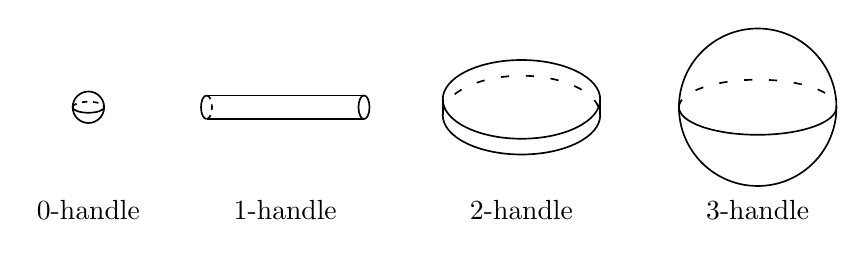
\begin{tikzpicture}[line width=.6, baseline=(base.base)]
    \tikzstyle{dp}=[dash pattern=on 2pt off 2pt]
    \draw (0,0) circle (.2);
    \draw[dp] (-.2,0) arc (180 : 0 : .2 and .07);
    \draw (-.2,0) arc (180 : 360 : .2 and .07);
    \node at (0,-1.3) {\text{$0$-handle}};
    
    \draw (1.5,.15) arc (90 : 270 : .07 and .15);
    \draw[dp] (1.5,.15) arc (90 : -90 : .07 and .15);
    \draw (3.5,0) ellipse (.07 and .15);
    \draw (1.5,.15) -- (3.5,.15) (1.5,-.15) -- (3.5,-.15);
    \node at (2.5,-1.3) {\text{$1$-handle}};

    \draw (5.5,.1) ellipse (1 and .5);
    \draw[loosely dashed] (4.5,-.1) arc (180 : 0 : 1 and .5);
    \draw (4.5,-.1) arc (180 : 360 : 1 and .5);
    \draw (4.5,.1) -- (4.5,-.1) (6.5,.1) -- (6.5,-.1);
    \node at (5.5,-1.3) {\text{$2$-handle}};

    \draw (8.5,0) circle (1);
    \draw[loosely dashed] (7.5,0) arc (180 : 0 : 1 and .35);
    \draw (7.5,0) arc (180 : 360 : 1 and .35);
    \node (base) at (8.5,-1.3) {\text{$3$-handle}};
\end{tikzpicture} \]

Every manifold can be obtained from $0$-handles
by attaching other handles.
For example, the solid torus $D^2 \times S^1$
decomposes into a $0$-handle and a $1$-handle.
\[ 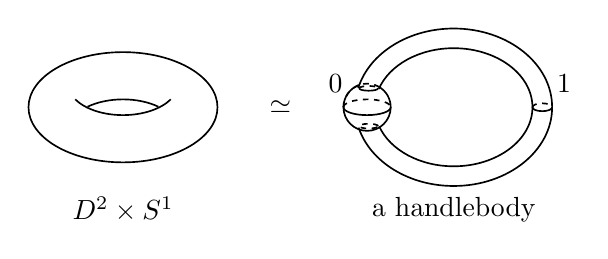
\begin{tikzpicture}[line width=.6]
    \tikzstyle{dp}=[dash pattern=on 2pt off 2pt]
    \draw (0,0) ellipse (1.2 and .7);
    \draw (0,-.1) arc (-90 : -30 : .7 and .4);
    \draw (0,-.1) arc (-90 : -150 : .7 and .4);
    \draw (0,.1) arc (90 : 50 : .7 and .4);
    \draw (0,.1) arc (90 : 130 : .7 and .4);
    
    \node at (2,0) {\text{$\simeq$}};

    \draw[dp] (2.8,0) arc (180 : 50 : .3);
    \draw (2.8,0) arc (180 : 110 : .3);
    \draw (2.8,0) arc (180 : 420 : .3);
    \draw[dp] (2.8,0) arc (180 : 0 : .3 and .1);
    \draw (2.8,0) arc (180 : 360 : .3 and .1);

    \draw (5.45,0) arc (0 : 166 : 1.25 and 1);
    \draw (5.45,0) arc (0 : -165 : 1.25 and 1);
    \draw (5.2,0) arc (0 : 162 : 1 and .75);
    \draw (5.2,0) arc (0 : -161 : 1 and .75);

    \draw[dp] (3,.24) arc (180 : 0 : .12 and .03);
    \draw (3,.24) arc (180 : 360 : .12 and .03);
    \draw[dp] (3.12,-.24) ellipse (.12 and .03);
    \draw[dp] (5.2,0) arc (180 : 0 : .125 and .05);
    \draw (5.2,0) arc (180 : 360 : .125 and .05);

    \node at (0,-1.3) {\text{$D^2 \times S^1$}};
    \node at (4.2,-1.3) {\text{a handlebody}};
    \node at (2.7,.3) {\text{0}};
    \node at (5.6,.3) {\text{1}};
\end{tikzpicture} \]

A formal definition goes as follows.

\begin{definition}
    A \term{relative $n$-handlebody} is a sequence
    \[ A = N_0 \subset N_1 \subset \cdots \]
    of smooth $n$-manifolds, possibly with boundary,
    such that each $N_i$ is obtained from $N_{i-1}$
    by attaching a $\lambda$-handle:
    \[ N_i \simeq N_{i-1} \cup_{\Phi_i} h^\lambda, \]
    where $\lambda$ may vary with $i$, and the attaching map
    \[ \Phi_i \: \partial D^\lambda \times D^{n-\lambda} \to \partial N_{i-1} \]
    is a smooth embedding.
    We require local finiteness (see below), so that the space
    \[ N := \bigcup_i N_i \]
    is a smooth $n$-manifold.

    By abuse of language,
    the pair $(N,A)$ is called a \term{relative $n$-handlebody}.
    If $A=\emptyset$, then $N$ is called an \term{$n$-handlebody}.
    It is \term{finite} if the above sequence is finite.
\end{definition}

In the definition, \term{local finiteness} means that 
every point in $N$ has a neighbourhood that intersects 
with only finitely many handles.
This is needed to ensure that $N$ is a manifold.

This definition is a bit sloppy,
since attaching a handle will form corners on the manifold,
and one needs to eliminate them in each step.
We do not go into the details,
for which the reader is referred to \cite{wall}.

The handlebody was invented by Smale,
and played a magical role in his proof of the
generalised Poincar\'e conjecture \cite{smale}.

\begin{theorem}[Generalised Poincar\'e conjecture]
    If $n\geq6$, then every $n$-manifold
    homotopy equivalent to the $n$-sphere
    is homeomorphic to the $n$-sphere.
\end{theorem}

Note that ``homeomorphic'' can not be improved to ``diffeomorphic'',
since there exist different smooth structures on $S^7$.

The main step of the proof was the following.

\begin{theorem}[$h$-cobordism theorem]
    Suppose $M,N,W$ are simply connected compact manifolds, with $\dim W\geq6$ and 
    \[ \partial W = M \sqcup N. \]
    If the inclusions $M\hookrightarrow W$ and $N\hookrightarrow W$
    are homotopy equivalences, then there is a diffeomorphism
    \[ W \simeq M \times [0,1]. \]
\end{theorem}

\begin{proof}[Sketch of Proof]
    The proof of this theorem relies on the theory of handlebodies.
    We first decompose $W$ into handles,
    regarding it as obtained from $M$ by attaching handles.
    For dimensional reasons, $M$ is replaced by $M\times[0,1]$,
    which is a neighbourhood of $M$ in $W$.
    Then we manipulate these handles using the following two theorems.
    It turns out that everything can be cancelled out perfectly,
    leading to the desired diffeomorphism.
\end{proof}

The two theorems that were used in the proof 
of the $h$-cobordism theorem are the following.

\begin{theorem}[Rearrangement] \label{thm-rearrangement}
    Every finite handlebody can be rearranged,
    so that every $\lambda$-handle is attached on handles
    of type $<\lambda$.
\end{theorem}

\[ 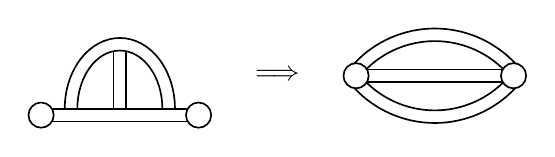
\begin{tikzpicture}[line width=.6]
    \draw (0,0) circle (.16);
    \draw (2,0) circle (.16);
    \draw (.14,.08) -- (1.86,.08) (.14,-.08) -- (1.86,-.08);
    \draw (.3,.08) arc (180 : 0 : .7 and .9);
    \draw (.46,.08) arc (180 : 0 : .54 and .74);
    \draw (.92,.08) -- (.92,.82) (1.08,.08) -- (1.08,.82);

    \node at (3,.5) {\text{$\Longrightarrow$}};

    \draw (4,.5) circle (.16);
    \draw (6,.5) circle (.16);
    \draw (4.14,.58) -- (5.86,.58) (4.14,.42) -- (5.86,.42);
    \draw (5,1.1) arc (90 : 137 : 1.4);
    \draw (5,1.1) arc (90 : 43 : 1.4);
    \draw (5,.94) arc (90 : 134 : 1.24);
    \draw (5,.94) arc (90 : 46 : 1.24);
    \draw (5,-.1) arc (-90 : -137 : 1.4);
    \draw (5,-.1) arc (-90 : -43 : 1.4);
    \draw (5,.06) arc (-90 : -134 : 1.24);
    \draw (5,.06) arc (-90 : -46 : 1.24);
\end{tikzpicture} \]

To be more precise,
it is convenient to introduce some terminology here.
(They are invented by the author and not meant to be used elsewhere.)

\begin{definition}
    Two $n$-handlebodies are \term{similar}
    if their manifolds $N$ are diffeomorphic, and for every $\lambda$,
    they have the same number of $\lambda$-handles.
\end{definition}

For example, the two handlebodies shown in the above picture are similar.

\begin{definition}
    A handlebody is \term{good} if 
    every $\lambda$-handle is attached on handles of type $<\lambda$.
\end{definition}

Thus, the rearrangement theorem can be reformulated as follows.

{
    \def\thetheorem{\ref*{thm-rearrangement}′}
    \begin{theorem}[Rearrangement]
        Every finite handlebody is similar to a good one.
    \end{theorem}
    \addtocounter{theorem}{-1}
}

The other theorem allows handles to cancel.

\begin{definition}
    The \term{belt} of the handle $D^\lambda \times D^{n-\lambda}$
    is $\{0\}\times \partial D^{n-\lambda}$,
    and the \term{cobelt} is $\partial D^\lambda\times\{0\}$.
    They are subsets of the boundary of the handle.
\end{definition}

\begin{theorem}[Cancellation]
    Suppose that 
    \[ N \cup h^\lambda \cup h^{\lambda+1} \]
    is a handlebody obtained from $N$ by attaching two handles.
    If the cobelt of $h^{\lambda+1}$ intersects the belt of $h^\lambda$
    in exactly one point,
    then the new handlebody is diffeomorphic to $N$.
\end{theorem}

\[ 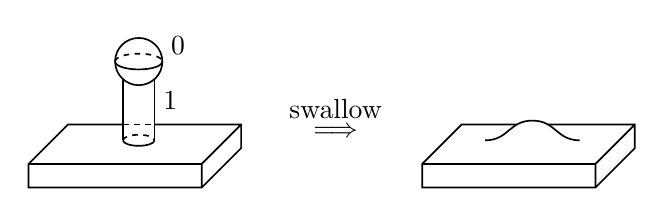
\begin{tikzpicture}[line width=.6]
    \tikzstyle{dp}=[dash pattern=on 2pt off 2pt]
    
    \draw (-.2,.2) -- (-.9,.2) -- (-1.4,-.3) -- (-1.4,-.6) -- (.8,-.6) -- (1.3,-.1) -- (1.3,.2) -- (.2,.2)
          (-1.4,-.3) -- (.8,-.3) -- (1.3,.2)
          (.8,-.3) -- (.8,-.6);
    \draw[dp] (-.2,.2) -- (.2,.2);

    \draw[dp] (-.2,0) arc (180 : 0 : .2 and .07);
    \draw (-.2,0) arc (180 : 360 : .2 and .07);
    \draw (-.2,0) -- (-.2,.78) (.2,0) -- (.2,.78);

    \draw (0,1) circle (.3);
    \draw[dp] (-.3,1) arc (180 : 0 : .3 and .1);
    \draw (-.3,1) arc (180 : 360 : .3 and .1);

    \node at (.5,1.2) {0};
    \node at (.4,.5) {1};

    \node at (2.5,.1) {\text{$\Longrightarrow$}};
    \node at (2.5,.4) {\text{swallow}};
    
    \draw (4.8,.2) -- (4.1,.2) -- (3.6,-.3) -- (3.6,-.6) -- (5.8,-.6) -- (6.3,-.1) -- (6.3,.2) -- (5.2,.2)
          (3.6,-.3) -- (5.8,-.3) -- (6.3,.2)
          (5.8,-.3) -- (5.8,-.6);
    \draw (4.4,0) .. controls (4.7,0) and (4.7,.25) .. (5,.25)
                  .. controls (5.3,.25) and (5.3,0) .. (5.6,0);
\end{tikzpicture} \]
\[ 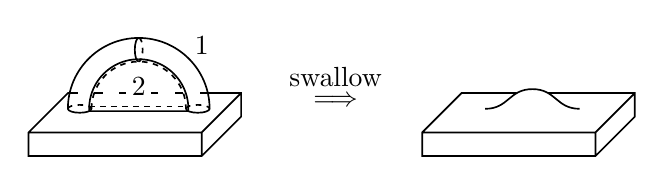
\begin{tikzpicture}[line width=.6]
    \tikzstyle{dp}=[dash pattern=on 2pt off 2pt]
    
    \draw (-.88,.2) -- (-.9,.2) -- (-1.4,-.3) -- (-1.4,-.6) -- (.8,-.6) -- (1.3,-.1) -- (1.3,.2) -- (.88,.2)
          (-1.4,-.3) -- (.8,-.3) -- (1.3,.2)
          (.8,-.3) -- (.8,-.6)
          (-.63,-.03) -- (.63,-.03);
    \draw[loosely dashed] (.88,.2) -- (0,.2) (-.88,.2) -- (0,.2);
    \draw[dp] (-.63,.03) -- (.63,.03);

    \draw[dp] (-.9,0) arc (180 : 0 : .15 and .05);
    \draw (-.9,0) arc (180 : 360 : .15 and .05);
    \draw[dp] (.6,0) arc (180 : 0 : .15 and .05);
    \draw (.6,0) arc (180 : 360 : .15 and .05);
    \draw[dp] (0,.9) arc (90 : -90 : .05 and .15);
    \draw (0,.9) arc (90 : 270 : .05 and .15);
    \draw (-.9,0) arc (180 : 0 : .9);
    \draw[dp] (-.6,0) arc (180 : 0 : .6);
    \draw (0,.63) arc (90 : -2 : .63);
    \draw (0,.63) arc (90 : 182 : .63);

    \node at (.8,.8) {1};
    \node[fill=white, inner xsep=2pt] at (0,.28) {2};

    \node at (2.5,.1) {\text{$\Longrightarrow$}};
    \node at (2.5,.4) {\text{swallow}};
    
    \draw (4.8,.2) -- (4.1,.2) -- (3.6,-.3) -- (3.6,-.6) -- (5.8,-.6) -- (6.3,-.1) -- (6.3,.2) -- (5.2,.2)
          (3.6,-.3) -- (5.8,-.3) -- (6.3,.2)
          (5.8,-.3) -- (5.8,-.6);
    \draw (4.4,0) .. controls (4.7,0) and (4.7,.25) .. (5,.25)
                  .. controls (5.3,.25) and (5.3,0) .. (5.6,0);
\end{tikzpicture} \]

For the proofs of these theorems,
see \cite{matsu} or \cite{milnor2}.
\medskip

Handlebodies are ubiquitous in the following sense.

\begin{theorem}\label{cor:handle-decomp}
    Every manifold is diffeomorphic to a good handlebody.
\end{theorem}

\begin{proof}
    \cite[Corollary~5.2.2]{wall}.
\end{proof}

However, some powerful tools, such as the rearrangement theorem,
fail for infinite handlebodies.
For example, consider the $2$-dimensional handlebody depicted below.
\[ 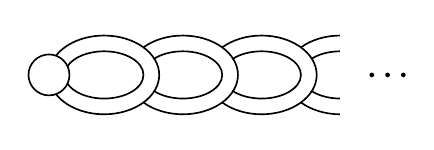
\begin{tikzpicture}[line width=.6]
    \draw (0,0) circle (.26);
    \draw (1.4,0) arc (0 : 151 : .7 and .5);
    \draw (1.4,0) arc (0 : -151 : .7 and .5);
    \draw (1.2,0) arc (0 : 159 : .5 and .3);
    \draw (1.2,0) arc (0 : -159 : .5 and .3);
    \draw (2.4,0) arc (0 : 136 : .7 and .5);
    \draw (2.4,0) arc (0 : -136 : .7 and .5);
    \draw (2.2,0) arc (0 : 138 : .5 and .3);
    \draw (2.2,0) arc (0 : -138 : .5 and .3);
    \draw (3.4,0) arc (0 : 136 : .7 and .5);
    \draw (3.4,0) arc (0 : -136 : .7 and .5);
    \draw (3.2,0) arc (0 : 138 : .5 and .3);
    \draw (3.2,0) arc (0 : -138 : .5 and .3);
    \draw (4.4,0) arc (0 : 136 : .7 and .5);
    \draw (4.4,0) arc (0 : -136 : .7 and .5);
    \draw (4.2,0) arc (0 : 138 : .5 and .3);
    \draw (4.2,0) arc (0 : -138 : .5 and .3);
    \fill[white] (3.7,.6) rectangle (4.5,-.6);
    \fill (4.1,0) circle (.03);
    \fill (4.3,0) circle (.03);
    \fill (4.5,0) circle (.03);
\end{tikzpicture} \]
If this handlebody were similar to a good handlebody,
then infinitely many $1$-handles would be attached
on the $0$-handle simultaneously,
so that the local finiteness criterion would fail.
In other words, if we attach handles in that way (pictured below),
we would get a topological space that is not a manifold.
\[ 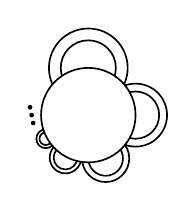
\begin{tikzpicture}[line width=.6]
    \draw[fill=white] (0,.6) circle (.5);
    \draw[fill=white] (0,.6) circle (.35);
    \draw[fill=white] (.6,0) circle (.4);
    \draw[fill=white] (.6,0) circle (.3);
    \draw[fill=white] (.22,-.55) circle (.3);
    \draw[fill=white] (.22,-.55) circle (.22);
    \draw[fill=white] (-.29,-.54) circle (.2);
    \draw[fill=white] (-.29,-.54) circle (.15);
    \draw[fill=white] (-.54,-.3) circle (.12);
    \draw[fill=white] (-.54,-.3) circle (.08);
    \draw[fill=white] (0,0) circle (.6);
    \fill (-.7, -.1) circle (.03);
    \fill (-.72, 0) circle (.03);
    \fill (-.74, .1) circle (.03);
\end{tikzpicture} \]

The purpose of this paper
is to introduce a variant of the notion of handlebodies,
which accepts this kind of spaces as handlebodies.
We will prove the rearrangement and cancellation theorems 
for this kind of handlebodies.
These results will make handle theory 
more available to non-compact manifolds.


\section{Weak handlebodies}

Here is the definition of our new notion of a handlebody.

\begin{definition}
    A \term{weak relative $n$-handlebody} is a finite or infinite sequence 
    \[ A=N_0\subset N_1\subset\cdots \]
    of $n$-manifolds,
    such that each $N_i$ is obtained from $N_{i-1}$ by attaching
    (finitely or infinitely many) handles of the same type, i.e.,
    \[ N_i \simeq N_{i-1} \cup_{\Phi_i} \biggl(\coprod_\alpha h^\lambda\biggr), \]
    where the attaching map
    \[ \Phi_i \: \coprod_\alpha {} \bigl( \partial D^\lambda\times D^{n-\lambda} \bigr) \to \partial N_{i-1} \]
    is required to be a closed embedding,
    which can be interpreted as \term{stepwise local finiteness}.
    Thus the space 
    \[ N:=\limdct{}(N_i\setminus\partial N_i) \]
    is a smooth manifold without boundary.
\end{definition}

By abuse of language, we say that $(N,A)$ is a weak relative handlebody.
If $A=\emptyset$, then we say that $N$ is a \term{weak handlebody}.

The weak handlebody discards information about the boundary.
However, this makes no difference when we talk about manifolds without boundary.

Moreover, it becomes possible for the 
rearrangement theorem to be true.

\begin{theorem}[Rearrangement] \label{thm-rearrange-weak}
Every weak relative handlebody
is similar to a good weak relative handlebody.
\end{theorem}

\[ 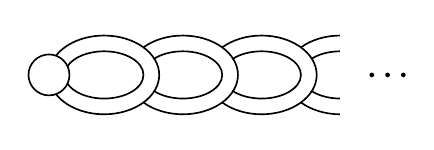
\begin{tikzpicture}[line width=.6, baseline=(base.base)]
    \draw (0,0) circle (.26);
    \draw (1.4,0) arc (0 : 151 : .7 and .5);
    \draw (1.4,0) arc (0 : -151 : .7 and .5);
    \draw (1.2,0) arc (0 : 159 : .5 and .3);
    \draw (1.2,0) arc (0 : -159 : .5 and .3);
    \draw (2.4,0) arc (0 : 136 : .7 and .5);
    \draw (2.4,0) arc (0 : -136 : .7 and .5);
    \draw (2.2,0) arc (0 : 138 : .5 and .3);
    \draw (2.2,0) arc (0 : -138 : .5 and .3);
    \draw (3.4,0) arc (0 : 136 : .7 and .5);
    \draw (3.4,0) arc (0 : -136 : .7 and .5);
    \draw (3.2,0) arc (0 : 138 : .5 and .3);
    \draw (3.2,0) arc (0 : -138 : .5 and .3);
    \draw (4.4,0) arc (0 : 136 : .7 and .5);
    \draw (4.4,0) arc (0 : -136 : .7 and .5);
    \draw (4.2,0) arc (0 : 138 : .5 and .3);
    \draw (4.2,0) arc (0 : -138 : .5 and .3);
    \fill[white] (3.7,.6) rectangle (4.5,-.6);
    \fill (4.1,0) circle (.03);
    \fill (4.3,0) circle (.03);
    \fill (4.5,0) circle (.03);
    \node (base) at (0,-.1) {};
\end{tikzpicture}
\qquad\Longrightarrow\qquad
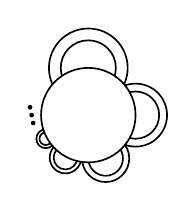
\begin{tikzpicture}[line width=.6, baseline=(base.base)]
    \draw[fill=white] (0,.6) circle (.5);
    \draw[fill=white] (0,.6) circle (.35);
    \draw[fill=white] (.6,0) circle (.4);
    \draw[fill=white] (.6,0) circle (.3);
    \draw[fill=white] (.22,-.55) circle (.3);
    \draw[fill=white] (.22,-.55) circle (.22);
    \draw[fill=white] (-.29,-.54) circle (.2);
    \draw[fill=white] (-.29,-.54) circle (.15);
    \draw[fill=white] (-.54,-.3) circle (.12);
    \draw[fill=white] (-.54,-.3) circle (.08);
    \draw[fill=white] (0,0) circle (.6);
    \fill (-.7, -.1) circle (.03);
    \fill (-.72, 0) circle (.03);
    \fill (-.74, .1) circle (.03);
    \node (base) at (0,-.1) {};
\end{tikzpicture} \]

As before, two relative handlebodies are \term{similar},
if the pairs $(N,A)$ are diffeomorphic as pairs of manifolds,
and for every $\lambda$, they have the same number (possibly infinite)
of $\lambda$-handles.
A relative handlebody is \term{good},
if every $\lambda$-handle is attached on handles of type $<\lambda$, or on $A$.

The proof will be given in \S\ref{sec-proofs}.

The cancellation theorem is also true,
with some modifications.

\begin{theorem}[Cancellation] \label{thm-cancel-weak}
    If a weak handlebody has a collection of pairs of handles
    satisfying the condition for cancellation,
    then these pairs can be cancelled simultaneously.
\end{theorem}

\[ 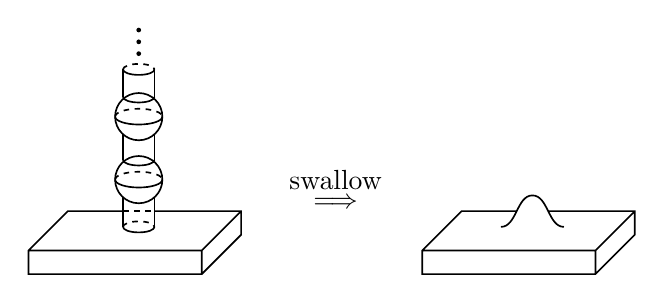
\begin{tikzpicture}[line width=.6]
    \tikzstyle{dp}=[dash pattern=on 2pt off 2pt]
    
    \draw (-.2,.2) -- (-.9,.2) -- (-1.4,-.3) -- (-1.4,-.6) -- (.8,-.6) -- (1.3,-.1) -- (1.3,.2) -- (.2,.2)
          (-1.4,-.3) -- (.8,-.3) -- (1.3,.2)
          (.8,-.3) -- (.8,-.6);
    \draw[dp] (-.2,.2) -- (.2,.2);

    \draw[dp] (-.2,0) arc (180 : 0 : .2 and .07);
    \draw (-.2,0) arc (180 : 360 : .2 and .07);
    \draw (-.2,0) -- (-.2,.38) (.2,0) -- (.2,.38);

    \draw (0,.6) circle (.3);
    \draw[dp] (-.3,.6) arc (180 : 0 : .3 and .1);
    \draw (-.3,.6) arc (180 : 360 : .3 and .1);

    \draw (-.2,.85) arc (180 : 360 : .2 and .07);
    \draw (-.2,.85) -- (-.2,1.18) (.2,.85) -- (.2,1.18);

    \draw (0,1.4) circle (.3);
    \draw[dp] (-.3,1.4) arc (180 : 0 : .3 and .1);
    \draw (-.3,1.4) arc (180 : 360 : .3 and .1);

    \draw (-.2,1.65) arc (180 : 360 : .2 and .07);
    \draw (-.2,1.65) -- (-.2,2) (.2,1.65) -- (.2,2);
    \draw (-.2,2) arc (180 : 360 : .2 and .07);
    \draw[dp] (-.2,2) arc (180 : 0 : .2 and .07);

    \fill (0,2.2) circle (.03);
    \fill (0,2.35) circle (.03);
    \fill (0,2.5) circle (.03);

    \node at (2.5,.3) {\text{$\Longrightarrow$}};
    \node at (2.5,.6) {\text{swallow}};
    
    \draw (4.8,.2) -- (4.1,.2) -- (3.6,-.3) -- (3.6,-.6) -- (5.8,-.6) -- (6.3,-.1) -- (6.3,.2) -- (5.2,.2)
          (3.6,-.3) -- (5.8,-.3) -- (6.3,.2)
          (5.8,-.3) -- (5.8,-.6);
    \draw (4.6,0) .. controls (4.8,0) and (4.8,.4) .. (5,.4)
                  .. controls (5.2,.4) and (5.2,0) .. (5.4,0);
\end{tikzpicture} \]

Precisely, \term{cancellation} means that the original handlebody is
diffeomorphic to a new handlebody, with the number of handles cut down.

A more precise formulation and the proof 
will be given as (\ref{thm:cancel-infinite}).


\section{Preliminaries on differential topology}

Simplicial sets arise from many topics in mathematics,
and they have a wide range of applications in various branches of mathematics.
For our purpose, they will be used as a model for $\infty$-categories,
as well as ordinary categories.
We will see how this is done in this section.

\subsection{Definition and examples}

Before giving the actual definition,
let us look at some examples of simplicial sets.

\begin{example}
    Let $X$ be a simplicial complex (as in topology),
    together with an ordering of vertices for each simplex $\sigma$,
    such that the inclusion of a face of $\sigma$ into $\sigma$
    preserves the ordering of vertices.
    Let $X_n$ denote the set of $n$-simplices of $X$, which may be degenerate.
    Then we have a series of maps
    \[\begin{tikzcd}
        \cdots\ar[r,shift left=3ex]\ar[r,shift left=1ex]\ar[r,shift right=1ex]\ar[r,shift right=3ex] &
        X_2\ar[l,shift left=2ex]\ar[l]\ar[l,shift right=2ex]\ar[r,shift left=2ex]\ar[r]\ar[r,shift right=2ex] &
        X_1\ar[l,shift left=1ex]\ar[l,shift right=1ex]\ar[r,shift left=1ex]\ar[r,shift right=1ex] &
        X_0\rlap{\ ,}\ar[l]
    \end{tikzcd}\]
    % \xymatrix{ \cdots\ar@<3ex>[r]\ar@<1ex>[r]\ar@<-1ex>[r]\ar@<-3ex>[r] & X_2\ar@<2ex>[l]\ar[l]\ar@<-2ex>[l]\ar@<2ex>[r]\ar[r]\ar@<-2ex>[r] & X_1\ar@<1ex>[l]\ar@<-1ex>[l]\ar@<1ex>[r]\ar@<-1ex>[r] & X_0\rlap{\ ,}\ar[l] }
    where $X_n$ has $(n+1)$ maps to $X_{n-1}$, called the \emph{face maps},
    defined by taking the $(n+1)$ faces of an $n$-simplex.
    $X_n$ also has $(n+1)$ maps to $X_{n+1}$, called the \emph{degeneracy maps},
    defined by regarding an $n$-simplex as a degenerate $(n+1)$-simplex.
    This structure is called a \emph{simplicial set}. \varqed
\end{example}

\begin{example}
    Let $X$ be a topological space, and denote
    \[\operatorname{Sing}(X)_n:=\Hom_{\cat{Top}}(\Delta^n,X),\]
    where $\Delta^n$ denotes the standard $n$-simplex in topology.
    Then $\operatorname{Sing}(X)$ is a simplicial set,
    having the same structure as in the previous example.
    This construction is used to define singular (co)homology in algebraic topology. \varqed
\end{example}

Now we will give the formal definition of a simplicial set.

\begin{definition}
    The category $\bfDelta$ is defined as follows.
    \begin{itms}
        \item Its objects are the sets $[n]:=\{0,\dotsc,n\}$ for all integers $n\geq0$.
        \item The hom-set $\Hom_\bfDelta([m],[n])$ consists of all maps from $[m]$ to $[n]$
              preserving the order $\leq$.
    \end{itms}
\end{definition}

In the category $\bfDelta$, there are two special classes of morphisms.
\begin{itms}
    \item There are $n$ maps from $[n]$ to $[n-1]$,
    denoted by $d^i$ $(0\leq i\leq n-1)$,
    defined by merging the elements $i$ and $i+1$ in $[n]$.
    These are called the \term{coface maps}.
    \item There are $(n+2)$ maps from $[n]$ to $[n+1]$,
    denoted by $s^i$ $(0\leq i\leq n+1)$,
    defined by skipping the element $i$ in $[n+1]$.
    These are called the \term{codegeneracy maps}.
\end{itms}
In fact, all morphisms in $\bfDelta$
can be written as a composition of these coface and codegeneracy maps.
These maps form a diagram
\[\begin{tikzcd}
    \relax[0]\ar[r] &
    \relax[1]\ar[l,shift left=1ex]\ar[l,shift right=1ex]\ar[r,shift left=1ex]\ar[r,shift right=1ex] &
    \relax[2]\ar[l,shift left=2ex]\ar[l]\ar[l,shift right=2ex]\ar[r,shift left=2ex]\ar[r]\ar[r,shift right=2ex] &
    \cdots\ar[l,shift left=3ex]\ar[l,shift left=1ex]\ar[l,shift right=1ex]\ar[l,shift right=3ex]
\end{tikzcd}\]
% \xymatrix{ [0]\ar[r] & [1]\ar@<1ex>[l]\ar@<-1ex>[l]\ar@<1ex>[r]\ar@<-1ex>[r] & [2]\ar@<2ex>[l]\ar[l]\ar@<-2ex>[l]\ar@<2ex>[r]\ar[r]\ar@<-2ex>[r] & \cdots\ar@<3ex>[l]\ar@<1ex>[l]\ar@<-1ex>[l]\ar@<-3ex>[l] }
in the category $\bfDelta$.

\begin{definition}
    A \term{simplicial set} is a functor from $\bfDelta\op$ to $\cat{Set}$,
    i.e.\ a contravariant functor from $\bfDelta$ to $\cat{Set}$.
    We denote the category of simplicial sets by
    \[\cat{sSet}:=\operatorname{Fun}(\bfDelta\op,\cat{Set}).\]
    More generally, for any category $\cat C$,
    a \term{simplicial object} in $\cat C$ is a functor from $\bfDelta\op$ to $\cat{C}$,
    and a \term{cosimplicial object} in $\cat C$ is a functor from $\bfDelta$ to $\cat{C}$.
\end{definition}

Let $X$ be a simplicial set.
The set $X_n:=X([n])$ is called the set of \term{$n$-simplices} of $X$.
The maps 
\[ d_i\:X_n\to X_{n-1}\quad\text{and}\quad s_i\:X_n\to X_{n+1},\quad\text{for }0\leq i\leq n, \]
induced by the morphisms $d^i$ and $s^i$ in the category $\bfDelta$,
are called the \term{face maps} and the \term{degeneracy maps}, respectively.

\begin{example}
    We construct some examples of simplicial sets.
    \begin{itms}
        \item The simplicial set $\Delta[n]$,
        as a simplicial complex, corresponds to the standard $n$-simplex.
        Its $k$-simplices are in 1--1 correspondence with 
        order-preserving maps $[k]\to[n]$,
        where $[n]$ can be seen as the set of vertices of $\Delta[n]$.
        \item Note that $\Delta[\bullet]$ is a cosimplicial object in $\cat{sSet}$.
        \item By removing the only non-degenerate $n$-simplex in $\Delta[n]$,
        we obtain its boundary $\partial\Delta[n]$.
        \item The simplicial set $S^n$ is defined to be $\Delta[n]\/\partial\Delta[n]$,
        where the quotient is done degreewise. \varqed
    \end{itms}
\end{example}

\begin{proposition}
    The category $\cat{sSet}$ admits all (small) colimits and limits, 
    which are defined degreewise, e.g.
    \[ (X\times Y)_n:=X_n\times Y_n. \]
\end{proposition}

\begin{proof}
    Exercise for the reader.
\end{proof}

For example, the product $\Delta[1]\times\Delta[1]$ is a solid square, which looks like
\[\begin{tikzcd}
    \bullet\ar[d]\ar[r]\ar[dr] & \bullet\ar[d] \\
    \bullet\ar[r] & \bullet\rlap{\ ,}
\end{tikzcd}\]
% \xymatrix{ \bullet\ar[d]\ar[r]\ar[dr] & \bullet\ar[d] \\ \bullet\ar[r] & \bullet\rlap{\ ,} }
with $2$ non-degenerate $2$-simplices and $5$ non-degenerate $1$-simplices,
but actually it has $3\times3=9=5+4$ possibly degenerate $1$-simplices in total.

\subsection{Geometric realisation}

A simplicial set is often pictured as
a simplicial complex together with an ordering of vertices for each simplex.
The idea of geometric realisation is that one can
forget the ordering and get a topological space.

\begin{proposition}
    Every simplicial set can be obtained from $\emptyset$
    by attaching $\Delta[n]$ along its boundary $\partial\Delta[n]$ and taking colimits. \qed
\end{proposition}

In the category $\cat{Top}$, we have the standard $n$-simplex $\Delta^n$.
If we put all these spaces together, we get a cosimplicial object $\Delta^\bullet$ in $\cat{Top}$,
which specifies ``how $\Delta[n]$ should look like in $\cat{Top}$''.
Given this data, we can easily define a functor
\[ |{\bullet}|\:\cat{sSet}\to\cat{Top} \]
by sending $\Delta[n]$ to $\Delta^n$,
and extending it to other simplicial sets by taking colimits.
This functor is called the \term{geometric realisation} functor.

Moreover, the functor $|{\bullet}|$ has a right adjoint called $\operatorname{Sing}$, defined by 
\[\operatorname{Sing}X:=\Hom_{\cat{Top}}(\Delta^\bullet,X),\]
which is exactly as we defined it before.

This construction can be generalised as follows.

\begin{construction}\label{con-3-a}
    Let $\cat C$ be a category with colimits.
    If we specify any cosimplicial object $\Delta^\bullet$ in $\cat{C}$,
    then we know ``how $\Delta[n]$ should look like in $\cat{C}$'',
    and we can similarly define an adjunction
    \[\begin{tikzcd}[column sep=5em]
        \cat{sSet}\ar[r,bend left=20,"\Delta{[n]}\mapsto\Delta^n"]\ar[r,phantom,"\bot"] &
        \rlap{$\cat{C}$\ .}\phantom{\cat{sSet}}\ar[l,bend left=20,"X\mapsto\Hom_{\cat C}(\Delta^\bullet\comma X)"]
    \end{tikzcd}\eqno◃\]
    % \xymatrix @C=5em {\cat{sSet}\ar@/^2ex/[r]^{\Delta{[n]}\mapsto\Delta^n}\ar@{}[r]|{\bot} & \rlap{\cat{C}\ .}\phantom{\cat{sSet}}\ar@/^2ex/[l]^{X\mapsto\Hom_{\cat C}(\Delta^\bullet,X)}}
\end{construction}

As we will see in the future,
many constructions related to simplicial sets are special cases of this construction.
Here is one example.

\begin{example}
    Let us take $\cat{C}=\cat{Ch}_R$, the category of cochain complexes of $R$-modules,
    where $R$ is a ring. Take
    \[\Delta^n:=\quad\Bigl(\cdots\to0\to
    \underset{\substack{\\[.5em](-n)}}{R^{\oplus\binom{n+1}{n+1}}}\to
    \cdots\to
    \underset{\substack{\\[.5em](-1)}}{R^{\oplus\binom{n+1}{2}}}\to
    \underset{\substack{\\[.5em](0)}}{R^{\oplus(n+1)}}\to0\to\cdots\Bigr)\]
    to be the simplicial chain complex of the standard $n$-simplex.
    This construction gives a functor $\cat{sSet}\to\cat{Ch}_R$,
    which computes the simplicial homology of a simplicial set.
    The composition
    \[\cat{Top}\xrightarrow{\operatorname{Sing}}\cat{sSet}\to\cat{Ch}_R\]
    computes the singular homology of a topological space. \varqed
\end{example}

Let us go back to the adjunction $|{\bullet}|\dashv\operatorname{Sing}$.
Actually, this is a Quillen equivalence between model categories.

\begin{definition}
    Let $0\leq i\leq n$.
    The simplicial set $\Lambda_i[n]$, called a \term{horn},
    is obtained from $\partial\Delta[n]$ by removing the face opposite to the $i$-th vertex.
\end{definition}

\begin{theorem}
    The category $\cat{sSet}$ has a \term{standard model structure}, with
    \begin{itms}
        \item $\cat W:=\{$weak homotopy equivalences of topological spaces$\}$.
        \item $\cat{Cof}:=\{$injections$\}$.
        \item $\cat{Fib}=\operatorname{RLP}\{\Lambda_i[n]\hookrightarrow\Delta[n]\mid0\leq i\leq n,\ n>0\}$.
        \item $\cat{Fib\cap W}=\operatorname{RLP}\{\partial\Delta[n]\hookrightarrow\Delta[n]\mid n\geq0\}$.
    \end{itms}
\end{theorem}

The proof is rather tedious and will not be presented here.
See~\cite[Theorem~3.6.5]{hovey}.

Finally, we state without proof the following result.

\begin{theorem}
    The adjunction $|{\bullet}|\dashv\operatorname{Sing}$
    is a Quillen equivalence between $\cat{sSet}$ and $\cat{Top}$.
\end{theorem}

See~\cite[Theorem 3.6.7]{hovey}.

The reader can show that the adjunction is a Quillen adjunction,
without using this theorem.

\subsection{Categories as simplicial sets}

Simplicial sets can be seen as a model for categories.
For example, the simplicial set $\Delta[2]$ can be seen as a diagram
\[\begin{tikzcd}[row sep=2em,column sep=1em]
    &\bullet\ar[dr] \\
    \bullet\ar[ur]\ar[rr]\ar[rr,phantom,bend left=45,"\Downarrow"] && \bullet\rlap{\ ,}
\end{tikzcd}\]
% \xymatrix @R=2em @C=1em{ &\bullet\ar[dr] \\ \bullet\ar[ur]\ar[rr]\ar@{}@/^2.5ex/[rr]|{\textstyle\Downarrow} && \bullet\rlap{\ ,} }
where the double arrow indicates that
the $2$-simplex ``witnesses'' the composition of the two arrows.
In an ordinary category, this diagram is just a chain of $2$ arrows
\[\bullet\to\bullet\to\bullet\ .\]
As another example, the simplicial set $\Delta[2]\times\Delta[1]$
corresponds to a diagram
\[\begin{tikzcd}
    \bullet\ar[d]\ar[r] & \bullet\ar[d]\ar[r] & \bullet\ar[d] \\
    \bullet\ar[r] & \bullet\ar[r] & \bullet\rlap{\ .}
\end{tikzcd}\]
% \xymatrix{ \bullet\ar[d]\ar[r] & \bullet\ar[d]\ar[r] & \bullet\ar[d] \\ \bullet\ar[r] & \bullet\ar[r] & \bullet\rlap{\ .} }

\begin{definition}
    Let $\cat C$ be a (small) category.
    The \term{nerve} of $\cat C$ is a simplicial set denoted by $\operatorname{N}(\cat C)$.
    Its $n$-simplices are chains of $n$ arrows
    \[\bullet\to\bullet\to\cdots\to\bullet\]
    in $\cat C$.
    Its $0$-th (resp.\ $n$-th) face map is defined by discarding the first arrow (resp.\ the last arrow).
    For $0<i<n$, its $i$-th face map is defined by composing its $i$-th and $(i+1)$-th maps.
    Its degeneracy maps are defined by inserting identity morphisms.
\end{definition}

The reader can verify that, in the above examples,
the nerve of the categories are the corresponding simplicial sets.

\begin{remark}
    In fact, this is another special case of (\ref{con-3-a}).
    Namely, the cosimplicial object $\Delta^\bullet$ in $\cat{Cat}$, given by 
    \[\Delta^n:=\quad\bullet\to\bullet\to\cdots\to\bullet\]
    with $n$ consecutive arrows, gives an adjunction
    \[\begin{tikzcd}
        \cat{sSet}\ar[r,bend left=30,"\Ho"]\ar[r,phantom,"\bot"] &
        \rlap{$\cat{Cat}$\ .}\phantom{\cat{sSet}}\ar[l,bend left=30,"\operatorname{N}"]
    \end{tikzcd}\]
    % \xymatrix{ \cat{sSet}\ar@/^/[r]^{\Ho}\ar@{}[r]|{\bot} & \cat{Cat}\rlap{\ .}\ar@/^/[l]^{\operatorname{N}} }
    The right adjoint is precisely the nerve functor defined above. \varqed
\end{remark}

Note that not all simplicial sets are categories.
For example, consider $\Lambda_1[2]$, which has two arrows that cannot be composed.
In fact, if we define the \term{spine} $\operatorname{Sp}(n)\subset\Delta[n]$
to consist of all vertices and the edges $[i,i+1]$ for $0\leq i<n$,
then a simplicial set $X$ is the nerve of a category,
if and only if it satisfies the lifting property
\[\begin{tikzcd}
    \operatorname{Sp}(n)\ar[d,hook]\ar[r] & X \\
    \Delta[n]\ar[ur,dashed,"\exists!"']
\end{tikzcd}\]
% \xymatrix{ \operatorname{Sp}(n)\ar[d]\ar[r] & X \\ \Delta[n]\ar@{-->}[ur] }
for all $n\geq 0$.

\subsection{Kan complexes and quasi-categories}

Kan complexes are simplicial sets that looks like topological spaces,
and will be used to model $\infty$-groupoids.

\begin{definition}
    A \term{Kan complex} is a fibrant simplicial set.
    In other words, it satisfies the \term{horn extension property},
    that is, the lifting property
    \[\begin{tikzcd}
        \Lambda_i[n]\ar[d,hook]\ar[r] & X \\
        \Delta[n]\ar[ur,dashed]
    \end{tikzcd}\]
    % \xymatrix{ \Lambda_i[n]\ar[d]\ar[r] & X \\ \Delta[n]\ar@{-->}[ur] }
    for all $0\leq i\leq n$, $n>0$.
\end{definition}


\begin{example}
    The simplicial set $\Delta[n]$ is \emph{not} a Kan complex if $n\geq1$.
    Namely, consider the horn
    \[\begin{aligned}
        \Lambda_0[2] &\to \Delta[n], \\
        0,1,2 &\mapsto 0,1,0.
    \end{aligned}\]
    Then it is impossible to extend this horn to make a $\Delta[2]$.
    The reason is that $\Delta[n]$, seen as a category,
    does not have inverses of morphisms. In other words, it does not look like a groupoid,
    while Kan complexes must look like groupoids. \varqed
\end{example}

\begin{example}
    For any topological space $X$, the simplicial set $\operatorname{Sing}X$
    is a Kan complex, as one can show easily.
    Therefore, for any simplicial set $S$, the simplicial set
    $\operatorname{Sing}|S|$
    can be used as a fibrant replacement of $S$. \varqed
\end{example}

As we have seen above, Kan complexes look like groupoids with higher structures.
In a Kan complex, $1$-morphisms are invertible,
but only up to a $2$-morphism, i.e.\ $2$-simplex.
The horn extension property ensures that all higher morphisms
are also invertible, up to even higher morphisms.
This is exactly what an $\infty$-groupoid should be.

\begin{definition}
    An \term{$\infty$-groupoid}, or an \term{$(\infty,0)$-category},
    is a Kan complex.
\end{definition}

For example, for a topological space $X$,
the Kan complex $\operatorname{Sing}X$ can be seen as 
the ``fundamental $\infty$-groupoid'' of $X$.

\begin{definition}
    A \term{homotopy type} is a homotopy type of $\infty$-groupoids,
    i.e.\ an element of $\Ho(\cat{sSet})$, which is equivalent to the category
    $\Ho(\cat{Top})\simeq\cat{hCW}$.
\end{definition}

Next, we wish to define $(\infty,1)$-categories in a similar way.
The following table shows that the extension of horns corresponds to 
properties of a category,
assuming that we are considering the nerve of an ordinary category.
\begin{center}
    \begin{tabular}{cc}
        \textbf{Horn} & \textbf{Property} \\ \hline
        $\Lambda_0[2]$ & every morphism is left invertible \\
        $\Lambda_1[2]$ & composition of morphisms \\
        $\Lambda_2[2]$ & every morphism is right invertible \\
        $\Lambda_0[3]$ & every morphism is an epimorphism \\
        $\Lambda_1[3]$, $\Lambda_2[3]$ & associativity of composition \\
        $\Lambda_3[3]$ & every morphism is a monomorphism \\
        otherwise & (satisfied by any category)
    \end{tabular}
\end{center}
As an exercise, the reader should verify everything in the table.

We notice that the extension of
$\Lambda_0[2]$, $\Lambda_2[2]$, $\Lambda_0[3]$ and $\Lambda_3[3]$
can not be satisfied by all categories,
while the extension of ``inner horns'' $\Lambda_i[n]$ for $0<i<n$
describes properties that any category should satisfy.

\begin{definition}
    A \term{quasi-category}, or an \term{$(\infty,1)$-category},
    is a simplicial set having the lifting property
    \[\begin{tikzcd}
        \Lambda_i[n]\ar[d,hook]\ar[r] & X \\
        \Delta[n]\ar[ur,dashed]
    \end{tikzcd}\]
    % \xymatrix{ \Lambda_i[n]\ar[d]\ar[r] & X \\ \Delta[n]\ar@{-->}[ur] }
    for $0<i<n$. In other words, \term{inner horns} can be extended.
\end{definition}

The terminology is that quasi-categories are 
one of the various models for $(\infty,1)$-categories.
For this reason, we will stick to the term ``quasi-categories''.
Some people also call quasi-categories ``weak Kan complexes''.

\subsection{Roadmap}

A number of models and tools for studying $(\infty,1)$-categories 
will be used in the sequel. 
Since we have finished most of the definitions,
it is a good point now to draw a roadmap
as a preview of what we will encounter.

For a monoidal category $\cat V$,
let $\cat{Cat}_{\cat V}$ denote the category of categories enriched over $\cat V$.
(We ignore the set-theoretic issues here.)
Let $\cat{Model}$ denote the category of model categories.
Let $\cat{Model}_{\cat V}$ denote the category of $\cat V$-enriched model categories,
which we have not defined yet.
Let $\cat{QsCat}$ denote the category of quasi-categories
(which should really be replaced by $\cat{sSet}$ in the following diagram).

We have a diagram of categories 
\[\begin{tikzcd}[row sep=1ex]
    \cat{Model} \ar[dd,"\text{localise}"']
    \ar[ddddr,start anchor={[xshift=-.5ex]west},bend right=90,"\Ho"'] &
    \cat{Model}_{\cat{sSet}} \ar[l,"\text{forget}"'] 
    \ar[dd,"\text{forget}"'] \\ 
%
    && \cat{Cat}_{\cat{sMod}_R} \ar[r,bend left=20,"\text{Dold--Kan}"]
    \ar[r,phantom,"\bot"]
    \ar[dl,bend left=20,start anchor={[xshift=-1.5ex,yshift=1ex]},
    end anchor={[yshift=1ex]},pos=.7,"\text{forget}" {rotate=25,inner sep=1pt}] &
    \rlap{$\cat{Cat}_{\cat{Ch}_R}$\scriptsize\enspace(dg categories)}
    \phantom{\cat{Cat}_{\cat{sMod}_R}} \ar[l,bend left=20] \\
%
    \cat{QsCat} \ar[r,bend left=20,"\mathfrak C"]
    \ar[r,phantom,"\bot\rlap{$\scriptstyle\simeq$}"] \ar[ddr,bend right,"h"'] &
    \cat{Cat}_{\cat{sSet}} \ar[l,bend left=20,"\mathfrak N"] \ar[dd,"h"']
    \ar[ur,bend left=20,start anchor={[xshift=1ex,yshift=1ex]},
    end anchor={[yshift=.5ex]},pos=.75,"\text{free}" rotate=25]
    \ar[ur,phantom,yshift=1ex,"\bot" rotate=25]
    \ar[dr,bend left=20,start anchor={[yshift=-1ex]},
    end anchor={[xshift=-1.5ex,yshift=-1ex]},pos=.45,"|\bullet|" {rotate=-22,inner sep=1pt}]
    \ar[dr,phantom,yshift=-1ex,"\bot\scriptstyle\simeq" rotate=-22] \\
    &&\cat{Cat}_{\cat{Top}} \ar[dl,bend left,"h"]
    \ar[ul,bend left=20,start anchor={[xshift=-1ex,yshift=-1ex]},
    end anchor={[xshift=.5ex,yshift=-1ex]},pos=.25,"\operatorname{Sing}" rotate=-22]\\
%
    &\cat{Cat}_{\cat{hCW}} \ar[dd,"\pi_0"] \\ \  \\
    &\cat{Cat}\rlap{\ .}
\end{tikzcd}\hspace{3em}\]
Some of the maps are easy to define, while others will be defined later.
This diagram is ``commutative'', in a sense which will be made precise later on.
Everything above $\cat{Cat}_{\cat{hCW}}$ can be seen as
models for $(\infty,1)$-categories.
Homotopy theory in these categories are called \term{homotopy coherent},
as opposed to \term{homotopy commutative}, 
which refers to commutative diagrams in $\cat{Cat}_{\cat{hCW}}$.

As we can see in the diagram, homological algebra, which is done in a dg (differential graded) category,
is related to $(\infty,1)$-category theory.
This relationship will be studied a few sections later.



\section{The proofs}

\label{sec-proofs}

This section is dedicated to the proofs of the
rearrangement theorem (\ref{thm-rearrange-weak}) and
the cancellation theorem (\ref{thm-cancel-weak})
for weak handlebodies.

\subsection{The rearrangement theorem}

\begin{definition}
    Let $M$ be a manifold.
    A smooth function $\theta\:M\to[0,1]$ is called a \term{level function},
    if $\theta^{-1}(0)=\partial M$ and $\theta$ has no critical points on $\partial M$.
\end{definition}

\begin{proposition}
    Every smooth manifold has a level function.
\end{proposition}

\begin{proof}
    Exercise for the reader.
\end{proof}

\begin{definition}
    Let $M$ be a manifold with a level function $\theta$, and let $\epsilon>0$.
    An \term{$\epsilon$-sliding} of $M$ is a diffeotopy $h\:M\times\R\to M$, such that
    \begin{enum}
        \item $h$ is supported in $\{p\in M\mid \theta(p)<\epsilon\}$.
        \item $\theta$ is preserved by $h$.
    \end{enum}
\end{definition}

Intuitively, an $\epsilon$-sliding moves the boundary around,
and keeps most of the interior fixed.
When we talk about an $\epsilon$-sliding,
we will implicitly assume that some level function $\theta$ is chosen.

\begin{lemma}\label{lem:slide}
Let $M$ be a manifold, and let $\epsilon>0$.
If $X$ is a compactly supported vector field on $\partial M$,
then $X$ can be extended to a vector field $\widetilde X$ on $M$,
which generates an $\epsilon$-sliding of $M$.
\end{lemma}

\begin{proof}
Let $U:=\{p\in M\mid \theta(p)<\epsilon\}$, 
where $\theta$ is the level function.
Let $K\subset\partial M$ denote the support of $X$.
Let $\partial M\times[0,+\infty)\subset M$ be a collar neighbourhood.
Since $K$ is compact,
we may assume $K\times[0,\epsilon]\subset U$.
We also assume that $\theta$ has no critical points in $K\times[0,\epsilon]$.

Let $\rho\:[0,+\infty)\to[0,1]$ be a smooth function such that
$\rho(0)=1$ and $\rho(r)=0$ when $r>\epsilon/2$.
We first extend $X$ to $M$ by letting
\[ X_p:=\biggl\{\mkern-3mu\begin{array}{ll}
\rho(r)\,X_q,&p=(q,r)\in K\times[0,\epsilon],\\
0,&\text{otherwise}.
\end{array} \]

Next we take a metric on $M$,
so that for all $p\in\partial M$, $\grad \theta(p)$ is orthogonal to $\T_p(\partial M)\subset\T_pM$.
This is possible by the constant rank theorem,
together with a partition of unity.
We define 
\[ \widetilde X:=X-\frac{\langle X,\grad \theta\rangle}{|\grad \theta|^2}\grad \theta. \]

Since $\widetilde X$ is supported in $K\times[0,\epsilon]$,
it generates a diffeotopy $h$.
Since $\widetilde X$ is orthogonal to $\grad\theta$,
$h$ is indeed an $\epsilon$-sliding. 
\end{proof}

\begin{remark}
If $X$ is instead supported in a disjoint union of countably many compact sets,
the lemma still holds true.
The reason is that the collar is global,
and will make sure that the sets $K\times[0,\epsilon]$ are disjoint.
\end{remark}

\begin{corollary}\label{cor:slide}
Every diffeotopy of $\partial M$ supported in
a disjoint union of compact sets 
can be extended to an $\epsilon$-sliding of $M$.
\end{corollary}

\begin{proof}
Apply (\ref{lem:slide}) to the velocity field of the diffeotopy.
This is a time-dependent vector field,
but the above proof applies as well.
\end{proof}

\begin{lemma}\label{lem:shrink}
    Let $(N,A)$ be a relative $n$-handlebody, 
    and let $\Phi\:\partial_1h^\lambda\to\partial N$ be an embedding,
    where $\lambda\neq0,n$.
    For any neighbourhood $U$ of the cobelt $\Phi(\partial D^\lambda\times0)$ in $\partial N$,
    the image of $\Phi$ can be moved into $U$ by an isotopy.
\end{lemma}
    
\begin{proof}
    Take any metric on $\partial N$.
    Then there exists $\epsilon>0$
    such that $\Phi(\partial D^\lambda\times\subsup D\epsilon{n-\lambda})\subset U$,
    where $\subsup D\epsilon{n-\lambda}$ denotes the disk of radius $\epsilon$.
    Now shrink $\Phi(\partial D^\lambda\times D^{n-\lambda})$ into this $\epsilon$-neighbourhood linearly.
\end{proof}

\begin{definition}
    Let $(N,A)$ be a weak relative $n$-handlebody, $i\geq0$ a fixed integer,
    and let $h\:N_i\to N_i$ be a diffeomorphism.
    The \term{perturbation by $h$} of $(N,A)$ is a relative handlebody $(N^h,A)$,
    with attaching maps $\Phi^h_j$, defined as follows:
    \begin{itms}
        \item $\subsup Njh=N_j$ and $\subsup\Phi jh=\Phi_j$ for all $j\leq i$.
        \item $\subsup\Phi{i+1}h=h\circ\Phi_{i+1}$. 
        This induces a diffeomorphism $h_{i+1}\:N_{i+1}\to\subsup N{i+1}h$.
        \item $\subsup\Phi{i+2}h=h_{i+1}\circ\Phi_{i+2}$,
        inducing a diffeomorphism $h_{i+2}\:N_{i+2}\to\subsup N{i+2}h$.
        \item And so on.
    \end{itms}
    The perturbation is called an \term{$\epsilon$-perturbation} if $h$ is an $\epsilon$-sliding.
    
    A finite composition of perturbations
    is also considered a perturbation.
\end{definition}

After a perturbation, the handles attached after the $i$-th step
will get attached to different handles,
but the new handlebody is similar to the original one.
We will see that every handlebody can be perturbed into a good one.

\begin{notation}
    Write
    \[ \partial_1h^\lambda := \partial D^\lambda \times D^{n-\lambda}
    \quad\text{and}\quad
    \partial_2h^\lambda := D^\lambda \times \partial D^{n-\lambda}, \]
    so that $\partial h^\lambda = \partial_1h^\lambda \cup \partial_2h^\lambda$.
    \varqed
\end{notation}

The idea of our proof of the rearrangement theorem 
is to create a vector field on the side of each handle,
so that other handles attached on it
can be slid out of it along this vector field.

\begin{definition}
    Let $h^\lambda$ be a $\lambda$-handle, where $\lambda\neq0,n$.
    Let $B\subset\partial_2h^\lambda$ be a closed subset,
    and let $O$ denote the belt of $h^\lambda$.
    An \term{expanding field} of $h^\lambda$ with respect to $B$
    is a vector field $X$ on $\partial_2h^\lambda$, such that
    \begin{itms}
        \item $X_p=0$ if and only if $p\in B\cup O$.
        %\item $X_p$ points outwards for $p\in\partial(\partial_2h^\lambda)-B$.
        \item For every $p\in\partial_2h^\lambda\setminus(B\cup O)$,
        the flow line of $X$ starting from $p$ reaches $\partial\partial_2h^\lambda$ within finite time.
    \end{itms}
    
    Let $(N,A)$ be a finite relative $n$-handlebody.
    Its \term{skeleton} is defined to be the set $\Sigma$ of compact submanifolds of $\partial N$,
    consisting of
    \begin{enum}
        \item The intersection of $\partial N$ with
        the boundary of the image of every attaching map.
        \item The intersection of $\partial N$ with
        the belt of each handle.
        \item All possible intersections of the manifolds listed above.
    \end{enum}
    In order for \textup{(iii)} to be well-defined, we require that
    the set of submanifolds in \textup{(i)} and \textup{(ii)} is transverse.
    Such a finite relative handlebody is said to be \term{regular}.
    We denote by $\Sigma_i$ the skeleton of $(N_i,A)$,
    and call it the \term{$i$-skeleton} of $(N,A)$.
    
    A regular $n$-handlebody $(N,A)$ is said to be \term{expanded},
    if every $\lambda$-handle $h^\lambda$ with $\lambda\neq0,n$ has an expanding field
    with respect to the union of images of attaching maps of handles
    that are attached after it.
\end{definition}

An expanding field does not necessarily exist for arbitrary $B$.
For example, consider the case $n=2$, $\lambda=1$ and $B$ is a point not in $O$.

The next lemma makes clear how expanding fields work.
The main idea of the proof is visualised below.
\[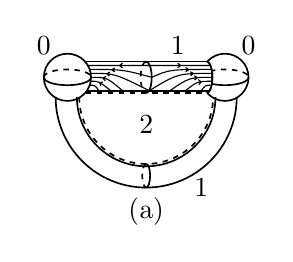
\begin{tikzpicture}[line width=.6, baseline=(base.base)]
    \tikzstyle{dp}=[dash pattern=on 2pt off 2pt]
    \draw (-1,0) circle (0.3);
    \draw (1,0) circle (0.3);
    \draw[dp] (-1.3,0) arc (180:0:0.3 and 0.1);
    \draw (-1.3,0) arc (180:360:0.3 and 0.1);
    \draw[dp] (.7,0) arc (180:0:0.3 and 0.1);
    \draw (.7,0) arc (180:360:0.3 and 0.1);
    \draw[dp,fill=white] (.77,0) ellipse (.07 and .2);
    \fill[white] (.72,0) ellipse (.07 and .2);
    \draw (-.77,.2) -- (.77,.2);
    \draw[dp] (-.77,-.2) -- (.77,-.2);
    \draw (-.75,-.17) -- (.8,-.17);
    \draw (.77,.2) arc (90:-90:.07 and .2);
    \draw (0,.2) arc (90:-90:.07 and .2);
    \draw[dp] (0,.2) arc (90:270:.07 and .2);
    \draw (-1.15,-.25) arc (180:360:1.15);
    \draw[dp] (-.85,-.25) arc (180:360:.85);
    \draw (-.88,-.25) arc (180:360:.88);
    \draw (0,-1.1) arc (90:-90:.05 and .15);
    \draw[dp] (0,-1.1) arc (90:270:.05 and .15);

    \draw[thin] (0,.15) -- (.82,.15) (.4,.18) -- (.44,.15) -- (.4,.12); 
    \draw[thin] (.07,0) .. controls (.3,.1) and (.3,.1) .. (.84,.1) (.5,.125) -- (.54,.095) -- (.5,.07);
    \draw[thin] (.04,-.17) .. controls (.4,.05) and (.4,.05) .. (.85,.05) (.56,.07) -- (.6,.05) -- (.565,.02);
    \draw[thin] (.3,-.17) .. controls (.55,0) and (.55,0) .. (.85,0) (.61,.02) -- (.65,-.005) -- (.615,-.035);
    \draw[thin] (.5,-.17) .. controls (.65,-.05) and (.65,-.05) .. (.85,-.05) (.66,-.03) -- (.7,-.057) -- (.67,-.095);
    \draw[thin] (.7,-.17) .. controls (.75,-.1) and (.75,-.1) .. (.84,-.1);
    
    \draw[thin] (.04,.15) -- (-.74,.15) (-.3,.18) -- (-.34,.15) -- (-.3,.12); 
    \draw[thin] (.07,0) .. controls (-.3,.1) and (-.3,.1) .. (-.72,.1) (-.4,.12) -- (-.44,.095) -- (-.4,.07);
    \draw[thin] (.04,-.17) .. controls (-.4,.05) and (-.4,.05) .. (-.7,.05) (-.46,.067) -- (-.5,.045) -- (-.465,.015);
    \draw[thin] (-.3,-.17) .. controls (-.5,0) and (-.5,0) .. (-.7,0) (-.51,.012) -- (-.55,-.008) -- (-.52,-.045);
    \draw[thin] (-.45,-.17) .. controls (-.6,-.05) and (-.6,-.05) .. (-.7,-.05) (-.55,-.06) -- (-.59,-.07) -- (-.575,-.11);
    \draw[thin] (-.6,-.17) .. controls (-.65,-.1) and (-.65,-.1) .. (-.72,-.1);

    \node at (0,-0.6) {2};
    \node at (.4,0.4) {1};
    \node at (.7,-1.4) {1};
    \node at (1.3,0.4) {0};
    \node at (-1.3,0.4) {0};
    \node (base) at (0,-1.7) {(a)};
\end{tikzpicture}
\qquad
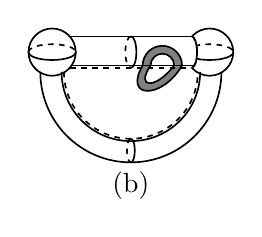
\begin{tikzpicture}[line width=.6, baseline=(base.base)]
    \tikzstyle{dp}=[dash pattern=on 2pt off 2pt]
    \fill[black!50] (.15,-.17) arc (180:0:.25);
    \fill[white] (.25,-.17) arc (180:0:.15);
    \fill[black!50] (.15,-.17) .. controls (-.1,-.6) and (.4,-.6) .. (.65,-.17);
    \fill[white] (.25,-.17) .. controls (.05,-.47) and (.32,-.47) .. (.55,-.17);
    \draw (-1,0) circle (0.3);
    \draw (1,0) circle (0.3);
    \draw[dp] (-1.3,0) arc (180:0:0.3 and 0.1);
    \draw (-1.3,0) arc (180:360:0.3 and 0.1);
    \draw[dp] (.7,0) arc (180:0:0.3 and 0.1);
    \draw (.7,0) arc (180:360:0.3 and 0.1);
    \draw[dp,fill=white] (.77,0) ellipse (.07 and .2);
    \fill[white] (.72,0) ellipse (.07 and .2);
    \draw (-.77,.2) -- (.77,.2);
    \draw[dp] (-.77,-.2) -- (.77,-.2);
    \draw (-.75,-.17) -- (.8,-.17);
    \draw (.77,.2) arc (90:-90:.07 and .2);
    \draw (0,.2) arc (90:-90:.07 and .2);
    \draw[dp] (0,.2) arc (90:270:.07 and .2);
    \draw (-1.15,-.25) arc (180:360:1.15);
    \draw[dp] (-.85,-.25) arc (180:360:.85);
    \draw (-.88,-.25) arc (180:360:.88);
    \draw (0,-1.1) arc (90:-90:.05 and .15);
    \draw[dp] (0,-1.1) arc (90:270:.05 and .15);
    \draw (.15,-.17) arc (180:0:.25);
    \draw (.25,-.17) arc (180:0:.15);
    \draw (.15,-.17) .. controls (-.1,-.6) and (.4,-.6) .. (.65,-.17);
    \draw (.25,-.17) .. controls (.05,-.47) and (.32,-.47) .. (.55,-.17);
    \node (base) at (0,-1.7) {(b)};
\end{tikzpicture}
\qquad
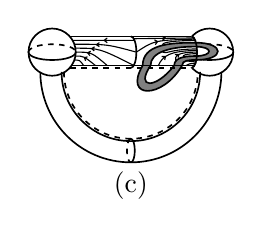
\begin{tikzpicture}[line width=.6, baseline=(base.base)]
    \tikzstyle{dp}=[dash pattern=on 2pt off 2pt]
    \draw (-1,0) circle (0.3);
    \draw (1,0) circle (0.3);
    \draw[dp] (-1.3,0) arc (180:0:0.3 and 0.1);
    \draw (-1.3,0) arc (180:360:0.3 and 0.1);
    \draw[dp] (.7,0) arc (180:0:0.3 and 0.1);
    \draw (.7,0) arc (180:360:0.3 and 0.1);
    \draw[dp,fill=white] (.77,0) ellipse (.07 and .2);
    \fill[white] (.72,0) ellipse (.07 and .2);
    \fill[black!50] (.15,-.17) .. controls (-.1,-.6) and (.4,-.6) .. (.65,-.17);
    \fill[white] (.25,-.17) .. controls (.05,-.47) and (.32,-.47) .. (.55,-.17);
    \fill[black!50] (.15,-.17) .. controls (.15,.1) and (.5,.12) .. (.82,.12)
    				 .. controls (1.2,.12) and (1.2,-.1) .. (.82,-.1)
    				 .. controls (.75,-.1) and (.65,-.1) .. (.65,-.17);
    \fill[white] (.25,-.17) .. controls (.25,0) and (.5,.07) .. (.82,.07)
    				 .. controls (1.05,.07) and (1.05,-.05) .. (.82,-.05)
    				 .. controls (.75,-.05) and (.55,-.05) .. (.55,-.17); 
    \draw (-.77,.2) -- (.77,.2);
    \draw[dp] (-.77,-.2) -- (.77,-.2);
    \draw (-.75,-.17) -- (.8,-.17);
    \draw (.77,.2) arc (90:-90:.07 and .2);
    \draw (0,.2) arc (90:-90:.07 and .2);
    \draw (-1.15,-.25) arc (180:360:1.15);
    \draw[dp] (-.85,-.25) arc (180:360:.85);
    \draw (-.88,-.25) arc (180:360:.88);
    \draw (0,-1.1) arc (90:-90:.05 and .15);
    \draw[dp] (0,-1.1) arc (90:270:.05 and .15);
    \draw (.15,-.17) .. controls (-.1,-.6) and (.4,-.6) .. (.65,-.17);
    \draw (.25,-.17) .. controls (.05,-.47) and (.32,-.47) .. (.55,-.17);
    \draw (.15,-.17) .. controls (.15,.1) and (.5,.12) .. (.82,.12)
    				 .. controls (1.2,.12) and (1.2,-.1) .. (.82,-.1)
    				 .. controls (.75,-.1) and (.65,-.1) .. (.65,-.17);
    \draw (.25,-.17) .. controls (.25,0) and (.5,.07) .. (.82,.07)
    				 .. controls (1.05,.07) and (1.05,-.05) .. (.82,-.05)
    				 .. controls (.75,-.05) and (.55,-.05) .. (.55,-.17); 
	\draw[thin] (.04,.15) -- (-.74,.15) (-.3,.18) -- (-.34,.15) -- (-.3,.12); 
    \draw[thin] (.07,0) .. controls (-.3,.1) and (-.3,.1) .. (-.72,.1) (-.4,.12) -- (-.44,.095) -- (-.4,.07);
    \draw[thin] (.04,-.17) .. controls (-.4,.05) and (-.4,.05) .. (-.7,.05) (-.46,.067) -- (-.5,.045) -- (-.465,.015);
    \draw[thin] (-.3,-.17) .. controls (-.5,0) and (-.5,0) .. (-.7,0) (-.51,.012) -- (-.55,-.008) -- (-.52,-.045);
    \draw[thin] (-.45,-.17) .. controls (-.6,-.05) and (-.6,-.05) .. (-.7,-.05) (-.55,-.06) -- (-.59,-.07) -- (-.575,-.11);
    \draw[thin] (-.6,-.17) .. controls (-.65,-.1) and (-.65,-.1) .. (-.72,-.1);

	\draw[thin] (.03,.17) -- (.8,.18) (.4,.2) -- (.44,.18) -- (.4,.15); 
	\draw[thin] (.07,0) .. controls (.3,.15) and (.3,.15) .. (.8,.165) (.3,.155) -- (.34,.135) -- (.31,.095);
	\draw[thin] (.4,.08) .. controls (.4,.11) and (.4,.14) .. (.82,.15);
	\draw[thin] (.4,0) .. controls (.45,-.03) and (.5,.04) .. (.84,.04);
	\draw[thin] (.35,-.17) .. controls (.4,-.05) and (.5,.02) .. (.84,.02) (.39,-.055) -- (.44,-.055) -- (.43,-.1);
	\draw[thin] (.57,-.12) .. controls (.55,-.04) and (.6,.0) .. (.84,.0) (.56,-.03) -- (.61,-.03) -- (.6,-.07);
	\draw[thin] (.67,-.06) .. controls (.65,-.04) and (.7,-.02) .. (.84,-.02);
	
	\draw[thin] (.7,-.11) .. controls (.75,-.125) and (.75,-.125) .. (.82,-.125);
    \draw[thin] (.7,-.17) .. controls (.75,-.145) and (.75,-.145) .. (.82,-.145);
    \node (base) at (0,-1.7) {(c)};
\end{tikzpicture}\]

\begin{center}
    \parbox{96mm}{\small\leftskip=1.5em\parindent=-1.5em
    (a) A $4$-handlebody, where numbers indicate types of handles.
    A $1$-handle is drawn with its expanding field.
    (Of course what is seen here is a $3$-dimensional analogue of the real thing.)
    
    (b) Attach a $3$-handle,
    where the shaded part indicates the image of the attaching map.
    
    (c) Stretch the attaching map using the expanding field,
    and construct a new expanding field on the $1$-handle.}\vspace{1pt}
\end{center}

\begin{lemma}\label{lem:expanded}
    Let $(N,A)$ be a finite relative $n$-handlebody with $i$ handles,
    such that $(N_{i-1},A)$ is good and expanded.
    Then $N_{i-1}$ can be $\epsilon$-slid,
    so that the induced $\epsilon$-perturbation is good and expanded.
\end{lemma}
    
\begin{proof}
    Let $h^\lambda$ denote the handle to be attached,
    and let $\Phi$ denote the attaching map.
    Let $h_j$ denote the handle attached in the $j$-th step.
    Since $(N_{i-1},A)$ is good, we may assume $h_1,\dotsc,h_{i-1}$ are of ascending types.
    
    First we try to slide $\image(\Phi)$ to avoid all handles of type $\geq\lambda$.
    Suppose $\image(\Phi)$ intersects with some $h_{\smash{j}}$ with type $\geq\lambda$,
    and we fix the largest $j$ with this property.
    Then $\image(\Phi)$ does not intersect with $h_{\smash{j+1}},\dotsc,h_{i-1}$.
    By reparametrising $h^\lambda$,
    we may assume that the cobelt $\Phi(\partial D^\lambda\times0)$ avoids the belt $O$ of $h_j$.
    By (\ref{lem:shrink}), we can shrink $\image(\Phi)$
    so that it does not meet $O$.
    We then extend the expanding field on $h_j$ to a small neighbourhood
    in $\partial N_j\cap\partial N_{i-1}$
    that does not meet any handles attached after the $j$-th step,
    and we could slide $\image(\Phi)$ out of $\partial_2h_j$
    using the flow $\phi_t$ of the expanding field for large enough $t$.
    We do this for all $h_j$, in descending order
    until $\image(\Phi)$ finally gets to a (literally) good position,
    i.e.\ within $\partial N_{i'-1}$, where
    $i'$ denotes the step where the first handle of type $\geq\lambda$ is attached.
    
    Our next plan is to do an $\epsilon$-sliding for each $j=i'-1,\dotsc,1$,
    making the corresponding handle expanded at each time.
    By (\ref{cor:transverse}), we may assume that
    $\Phi(\partial\partial_2h^{\lambda})$ is transverse to
    everything in $\Sigma_{i'-1}$,
    while keeping $\image(\Phi)$ disjoint with $h_{i'},\dotsc,h_{i-1}$.
    
    In the $j$-th step,
    let $X$ denote the expanding field on $\partial_2h_j$.
    Let $B\subset\partial N_j$ denote the union of images of attaching maps in steps $j+1,\dotsc,i-1$,
    intersected with $\partial N_j$.
    Let $\Phi'$ denote the composition of $\Phi$ with the previously executed slidings.
    
    Let $S_{j+1},\dotsc,S_i$
    be the boundaries of images of attaching maps
    in the corresponding steps, intersected with $\partial N_j$,
    so that $S_i=\Phi'(\partial\partial_2h^{\smash{\lambda}})\cap\partial N_j$.
    Let $O$ denote the belt of $h_j$.
    Thus the $S_k$ and $B$ are submanifolds possibly with corners,
    and the corners of $B$ are concave.
    By (\ref{lem:extension}) and the remark after it,
    we may extend the $S_k$ that have boundaries a little bit into $B$,
    so that the extended manifolds $\subsup Sk\prime$ are compact,
    and $\partial\subsup Sk\prime\subset B^\circ$ for all $k$.
    %(This can be achieved, for example, by projecting a compact collar of
    %$\partial\partial_2h_k$ in $\partial_2h_k$
    %to a collar of $\partial\partial_2h_k$ in $\partial N_{k-1}$ diffeomorphically,
    %and then projecting it to $\partial N_{k-2},\dotsc,$ and finally to $\partial N_j$.)
    
    By regularity of $(N_{i-1},A)$,
    we may assume $O,\subsup S{j+1}\prime,\dotsc,\subsup Si\prime$ are transverse
    (shrinking a bit the extended part if necessary).
    Thus by (\ref{cor:function}),
    there is a smooth function $f\:\partial N_j\setminus B^\circ\to[0,1]$,
    with $f^{\smash{-1}}(0)=(O\cup\subsup S{j+1}\prime\cup\cdots\cup\subsup Si\prime)\setminus B^\circ$,
    with no critical values other than $0,1$.
    We modify $f$ by letting $f|_B\equiv0$ and $f|_{\image(\Phi')}\equiv0$.
    Now $f$ becomes a smooth function $\partial N_j\to[0,1]$ with $f^{-1}(0)=O\cup B\cup\image(\Phi')$,
    and it has no critical values other than $0,1$.

    We extend $X$ to a compactly supported smooth vector field on $\partial N_j$,
    so that $X|_{B}=0$, and for any $p\in\partial\partial_2h_j$ such that $X_p\neq0$,
    the change of $f$ along the extended part of the flow line of $X$ through $p$ is $<1/2$.
    
    %Notice that any vector field $X'$ that is
    %close enough to $X$ in the sense of (\ref{lem:transversal})
    %is an expanding field.
    %Thus by (\ref{lem:transversal}), we may take such an expanding field $X'$,
    We take a large number $t\in\R$,
    such that the flow $h:=\phi_t$ of $X$ satisfies
    \[h\bigl(f^{-1}([1/2,1])\cap\partial_2h_j\bigr)\cap\partial_2h_j=\emptyset.\]
    By (\ref{cor:transverse}), after performing a small isotopy
    preserving the above condition, keeping $B$ fixed,
    we may assume that $h(\Phi'(\partial\partial_2h^\lambda))$ is transverse to
    everything in $\Sigma_{i-1}$.
    
    Take a metric on $\partial_2h_j$, and put
    \[ Y_p:=\d h(\grad f(h^{-1}(p))). \]
    One verifies that $Y$ is a new expanding field on $\partial_2h_j$, 
    but with respect to $B\cup\image(h\circ\Phi')$ instead of $B$.
    Note that $h$ keeps $B$ fixed.
    Finally we execute the $\epsilon$-sliding induced by $h$.
    
    We have finished the $j$-th step.
    Running over $j=i'-1,\dotsc,1$ gives a desired $\epsilon$-sliding,
    and gives desired expanding fields on all handles except the $i$-th one.
    But the $i$-th handle is trivially done.
    Regularity is preserved throughout the above construction.
\end{proof}

Having done much preparatory work,
we are finally ready to take our final step to proving (\ref{thm-rearrange-weak}),
namely, the concatenation of these infinitely many slidings
given by the preceding lemma.

\begin{proof}[Proof of \textup{(\ref{thm-rearrange-weak})}]
Let $(N,A)$ be a weak relative $n$-handlebody.
We may assume that only one handle is attached in each step.
For each $i\geq0$, we may regard $(N_i,A)$ as a non-weak relative handlebody.
Let $\theta_i$ be a level function on $N_i$ for $i=0,1,\dotsc$,
so that $\theta_i\leq\theta_{i+1}$ for all $i$.
%Denote $\subsup Ni\circ=N_i-\partial N_i$,
%and denote $\Theta(p):=\theta_i(p)$ if $p\in\subsup Ni\circ-\subsup N{i-1}\circ$,
%where $\subsup N{-1}\circ$ is understood to be the empty set.
%Thus $\Theta$ is a function 

Denote $N^1=N$. Note that $(\subsup N11,A)$ is automatically expanded.
By (\ref{lem:expanded}),
$\subsup N11$ can be $1/2$-slid,
so that if we denote by $(N^2,A)$ the induced perturbation,
then $(\subsup N22,A)$ is expanded. 
We continue to $1/4$-slide $\subsup N22$ to get a perturbation $(N^3,A)$ of $(N^2,A)$,
so that $(\subsup N33,A)$ is expanded.
Continuing this process, using $1/2^i$ in the $i$-th step,
we get a commutative grid of maps
\[ \begin{tikzcd}
\subsup N01\ar[r,hook] &\subsup N11\ar[r,hook]\ar[d,"\simeq"] &\subsup N21\ar[r,hook]\ar[d,"\simeq"] &\subsup N31\ar[r,hook]\ar[d,"\simeq"] &\subsup N41\ar[r,hook]\ar[d,"\simeq"] &\cdots\\
\subsup N02\ar[r,hook] &\subsup N12\ar[r,hook] &\subsup N22\ar[r,hook]\ar[d,"\simeq"] &\subsup N32\ar[r,hook]\ar[d,"\simeq"] &\subsup N42\ar[r,hook]\ar[d,"\simeq"] &\cdots\\
\subsup N03\ar[r,hook] &\subsup N13\ar[r,hook] &\subsup N23\ar[r,hook] &\subsup N33\ar[r,hook]\ar[d,"\simeq"] &\subsup N43\ar[r,hook]\ar[d,"\simeq"] &\cdots\rlap,\\
&&&\dots&\dots
\end{tikzcd} \]
where the vertical maps are all diffeomorphisms.
By construction $\subsup Nii$ and $\subsup Ni{i+1}$ are naturally identified,
but note that the identification is not the diffeomorphism (sliding) in the diagram.
We define $\theta_i$ on $\subsup N{\smash{j}}i$ for $i\leq j+1$ to be the
level function inherited from $N_j=\subsup Nj1$.
Thus for $\subsup Nii$ and $\subsup Ni{i+1}$,
their functions $\theta_i$ are the same under the natural identification.

We define a good weak relative $n$-handlebody $(N',A)$ 
by $\subsup Ni\prime:=\subsup Nii$, 
and the inclusion maps being $\subsup Nii=\subsup Ni{i+1}\hookrightarrow\subsup N{i+1}{i+1}$.
This is \emph{not} the map in the above diagram!
But for $p\in\subsup Nii\subset\subsup N{i+1}{i+1}$, we still have
$\theta_i(p)\leq\theta_{i+1}(p)$.
We will show that $N$ is diffeomorphic to $N'$. 

Consider the (not commutative) diagram
\[ \begin{tikzcd}
N_1\ar[d,equals]\ar[r,hook] &N_2\ar[d,"\simeq"]\ar[r,hook] &N_3\ar[d,"\simeq"]\ar[r,hook] &\cdots\\
\subsup N11\ar[r,hook] &\subsup N22\ar[r,hook] &\subsup N33\ar[r,hook] &\cdots\rlap,
\end{tikzcd}\eqno(*) \]
where the vertical maps are as in the above grid-like diagram.
By comparing the above two diagrams, the square
\[ \begin{tikzcd}
N_i\ar[r,hook]\ar[d,"\simeq"] &N_{i+1}\ar[d,"\simeq"]\\
\subsup Nii\ar[r,hook] &\subsup N{i+1}{i+1}
\end{tikzcd} \]
commutes for some $p\in N_i$
if and only if $p$ is fixed by the sliding $\subsup Nii\to\subsup Ni{i+1}$.
This happens whenever $\theta_i(p)>1/2^i$. Thus for
\[ U_i:=\{p\in N_i\mid\theta_i(p)>1/2^i\}, \]
the diagram $(*)$ commutes after the $i$-th square.
Thus we have an induced diffeomorphism of $U_i$ onto a subset of $N'$.
Since $N=\bigcup_{i=1}^\infty U_i$, we have an induced map $\phi\:N\to N'$
which is a diffeomorphism onto its image.
Clearly $\phi$ is also surjective since $N'=\bigcup_{i=1}^\infty\image(U_i\to N')$.
Thus $\phi$ is a diffeomorphism. 
\end{proof}

\subsection{The cancellation theorem}

We first state the cancellation theorem
for finite handlebodies.

\begin{theorem}[Cancellation, finite case]\label{thm:cancel}
Let $N=A\cup_{\Phi_1}h^\lambda\cup_{\Phi_2}h^{\lambda+1}$ be a relative handlebody with $2$ handles.
If the cobelt of $h^{\lambda+1}$ and the belt of $h^\lambda$ intersect transversely
at precisely one point, then $N$ is diffeomorphic to $A$.
This diffeomorphism can be taken to be fixed on any closed subset of $A\setminus\image(\Phi_1)\setminus\image(\Phi_2)$.
\end{theorem}

\begin{proof}
\cite[Theorem~5.4.3]{wall} or \cite[Theorem~3.34]{matsu}.
\end{proof}

For convenience, we introduce the following terminology.
In a good relative handlebody, a pair of $\lambda$- and $(\lambda+1)$-handles is called a
\term{cancelling pair}, if the cobelt of the $(\lambda+1)$-handle
and the belt of the $\lambda$-handle intersect transversely
at precisely one point. 
The $(\lambda+1)$-handle will be called the \term{canceller},
and the $\lambda$-handle will be called the \term{cancellee}.

We say that we can \term{cancel} a set $S$ of handles from a weak relative handlebody $(N,A)$,
if $N$ is diffeomorphic to a weak relative handlebody,
whose $\lambda$-handles correspond to
the $\lambda$-handles of $N$ that are not in $S$,
and the combinatorics concerning which handles are attached to other handles should not change,
except that a handle attached to a cancelled handle may get attached to
a handle which a cancelled handle was attached to.

\begin{theorem}[Cancellation, infinite case] \label{thm:cancel-infinite}
Let $(N,A)$ be a weak relative handlebody whose handles are attached one at a time,
and let $S$ be a set of handles consisting of cancelling pairs
that do not have handles in common,
such that every canceller in $S$ is attached immediately after its cancellee.
Then $S$ can be cancelled.
\end{theorem}

\begin{proof}
We will construct a new weak handlebody $N'$ diffeomorphic to $N$,
with the desired property.

Let $\subsup N0\prime:=N_0=A$, and let $\theta_0$ be a level function on it.
Let $\phi_0\:N_0\to\subsup N0\prime$ be a diffeomorphism.
As we construct $N'$, we will construct diffeomorphisms $\phi_i\:N_i\to\subsup Ni\prime$,
and level functions $\theta_i$ on $\subsup Ni\prime$,
such that $\theta_i\leq\theta_{i+1}$ on $\subsup Ni\prime$.
This will be implicit in the below construction.

In the $i$-th step, if the $i$-th handle of $N$ is not a canceller or a cancellee,
then we attach a same handle to $N'$ according to $\phi_{i-1}$,
and let $\phi_i$ be the induced diffeomorphism.
If it is a cancellee (followed by its canceller),
then we will not attach handles to $N'$ in the $i$-th and $(i+1)$-th steps.
Instead, we construct by (\ref{thm:cancel}) a diffeomorphism $\phi_{i+1}$ to form a (not commutative) diagram
\[ \begin{tikzcd}
N_{i-1}\ar[d,"\phi_{i-1}"',"\simeq"]\ar[r,hook] &N_i\ar[r,hook] &N_{i+1}\ar[d,"\phi_{i+1}"',"\simeq"]\\
\subsup N{i-1}\prime\ar[r,equals] &\subsup Ni\prime\ar[r,equals] &\subsup N{i+1}\prime\rlap.
\end{tikzcd} \]
By the last statement of (\ref{thm:cancel}), we may require the diagram to commute in
$\subsup U{i-1}\prime:=\{p\in\subsup N{i-1}\prime\mid\theta_{i-1}(p)>1/2^{i-1}\}$.
We take a new level function $\theta_{i+1}$ on $\subsup N{i+1}\prime$,
so that for all $p\in\subsup N{i-1}\prime$, we have
\[\theta_{i+1}(p)\geq\theta_{i-1}(p)\quad\text{and}\quad
\theta_{i+1}(p)\geq\theta_{i-1}(\phi_{i+1}\circ\subsup{\phi}{i-1}{-1}(p)).\]
By a same argument as before, we have a colimit map from $N'$ to $N$,
which is an embedding. It is surjective by the choice of the functions $\theta_i$.
\end{proof}

We have now completed the proof of our two 
main theorems. They can be combined to obtain
the following result, which simplifies weak handlebodies.

\begin{definition}
Let $n\geq m\geq0$ be integers. An \term{$(n,m)$-handlebody} is an $n$-handlebody
whose handles are of type $0,1,\dotsc,m$.
\end{definition}

\begin{corollary}\label{prop:0-handle}
Every connected finite handlebody is diffeomorphic to
a handlebody with only one $0$-handle.
Every connected weak handlebody is diffeomorphic to
a good weak handlebody with only one $0$-handle.
\end{corollary}

\begin{proof}
For the finite case, we may suppose that the handlebody is good by (\ref{thm-rearrangement}).
Thus it suffices to prove the statement for an $(n,1)$-handlebody.
Consider a graph with vertices corresponding to the $0$-handles
and edges corresponding to the $1$-handles.
Then this graph is connected.
Taking a maximal tree of this graph,
we may assume the handlebody is simply connected
(by discarding the $1$-handles not in the tree).
Thus the result follows from (\ref{thm:cancel}),
by cancelling the $0$- and $1$-handles a pair at a time.

For the weak case, we suppose that the handlebody is good by (\ref{thm-rearrange-weak}).
We construct a graph and take a maximal tree in the same way,
and the statement follows from (\ref{thm:cancel-infinite}).
\end{proof}


\section{Handle chain complexes}

One might notice the resemblance between a handlebody and a CW complex.
In fact, they are related in the following way.

\begin{definition}
Let $(N,A)$ be a good, weak or non-weak, relative handlebody.
We define its \term{associated CW complex} $(X,A)$ as follows.
Assume for $N$ that the handles are attached one at a time.
\begin{itms}
\item Let $X_0:=A$ as a trivial relative CW complex over $A$,
and let $p_0\:N_0\to X_0$ be the identity map.
\item If $N_1=N_0\cup_{\Phi_1}h^\lambda$,
we define $X_1:=X_0\cup_{\phi_1}D^\lambda$,
where $\phi_1:=p_0\circ\Phi_1|_{\partial D^\lambda\times 0}$.
We define a continuous map $p_1\:N_1\to X_1$ as follows.
Let $p_1$ agree with $p_0$ on $N_0$,
and let it be the projection to the core $D^\lambda\times0$ of $h^\lambda$.
\item We then define $X_2$ and $p_2$, and so on. 
\end{itms}
Thus $X:=\limdct X_i$ is a relative CW complex over $A$.
\end{definition}

\begin{proposition}\label{prop:ass-cw}
The associated CW complex is homotopy equivalent to the original, weak or non-weak, relative handlebody.
\end{proposition}

\begin{proof}
The weak case needs an extra first step. Note that $N_i$ is homotopy equivalent to $N_i\setminus\partial N_i$,
since if we take a collar neighbourhood $\partial N_i\times[0,+\infty)$,
then both spaces retract to $N_i\setminus\partial N_i\times[0,1)$.

We claim that each $p_i$ is a homotopy equivalence.
This is shown by induction on $i$. Since the projection onto the core is a homotopy equivalence
between $h^\lambda$ and $D^\lambda$, by \cite[Lemma~2.1.3]{may},
$N_i:=N_{i-1}\cup_{\Phi_i}h^\lambda$ and $X_i:=X_{i-1}\cup_{\phi_i}D^\lambda$
are homotopy equivalent through the induced map $p_i$.

Finally, by \cite[Lemma~2.1.10]{may}, the colimit map $p\:N\to X$ is a homotopy equivalence.
\end{proof}

As a consequence,
the (co)homology groups of a handlebody 
can be computed by the cellular (co)chain complex of 
its associated CW complex.
We shall define an analogous (co)chain complex associated to a handlebody.

\begin{definition}
Let $M,S,T$ be oriented $m$-, $s$- and $t$-manifolds without boundary,
with $S,T$ compact and $s+t=m$.
Let $f\:S\to M$, $g\:T\to M$ be embeddings.
If $f(S)$ is transverse to $g(T)$, then we define the
\term{intersection number} of $f,g$ to be
\[\#(f,g):=\sum_{p\in f(S)\cap g(T)}\pm1,\]
where the sign is decided by whether the vector space isomorphism
$\T_pM\simeq\T_pf(S)\oplus\T_pg(T)$
preserves $(+1)$ or reverses $(-1)$ the orientation.
\end{definition}

\begin{proposition}
Under the above assumptions, if $f$ is isotopic to $f'$ and $g$ is isotopic to $g'$,
such that $f'(S)$ is transverse to $g'(T)$, then $\#(f,g)=\#(f',g')$.
\end{proposition}

\begin{proof}
By (\ref{cor:isotopy-ext}), we may extend the isotopy from $g$ to $g'$ to an isotopy of $M$.
Thus we may assume $g=g'$.
For a proof in this case, see \cite[p.\,108]{gp}. 
\end{proof}

Therefore, the intersection number is well-defined for isotopy classes of maps.
This allows us to define the intersection number for submanifolds
that are not necessarily transverse.

\begin{definition}
Let $M,S,T$ be oriented $m$-, $s$- and $t$-manifolds without boundary,
where $S,T$ are compact submanifolds of $M$ with $s+t=m$.
Their \term{intersection number} $\#(S,T)$
is defined to be any $\#(f,g)$, such that $f$ is isotopic to the embedding $S\hookrightarrow M$,
$g$ is isotopic to $T\hookrightarrow M$, and $f(S)$ is transverse to $g(T)$.
\end{definition}

For any given $M,S,T$, such $f,g$ always exist.
This is a consequence of (\ref{cor:transverse}). 

\begin{definition}
Let $N$ be a good, weak or non-weak, $n$-handlebody,
and let $G$ be an abelian group.
The \term{handle chain complex} $C_\bullet(N;G)$ of $N$ is defined as follows.
\begin{itms}
\item $C_\lambda(N;G):=\bigoplus_\alpha G\cdot[\subsup h\alpha\lambda]$
for $\lambda=0,\dotsc,n$, and $0$ otherwise.
Here $\subsup h\alpha\lambda$ runs through all $\lambda$-handles of $N$.
\item $\partial_\lambda\:C_\lambda(N;G)\to C_{\lambda-1}(N;G)$ is defined on basis elements by
\[\partial_\lambda[\subsup h\alpha\lambda]:=\sum\#\bigl(\text{cobelt}(\subsup h\alpha\lambda),\ \text{belt}(\subsup h\beta{\lambda-1})\bigr)\,[\subsup h\beta{\lambda-1}],\]
where the sum is taken over all $(\lambda-1)$-handles $\subsup h\beta{\lambda-1}$
attached before $\subsup h\alpha\lambda$.
\end{itms}
If $N$ is locally finite, then we define the \term{handle cochain complex}
$C^\bullet(N;G)$ as follows.
\begin{itms}
\item $C^\lambda(N;G):=C_\lambda(N;G)$.
\item $d^\lambda\:C^\lambda(N;G)\to C^{\lambda+1}(N;G)$ is defined on basis elements by
\[d^\lambda[\subsup h\alpha\lambda]:=\sum\#\bigl(\text{belt}(\subsup h\alpha\lambda),\ \text{cobelt}(\subsup h\beta{\lambda+1})\bigr)\,[\subsup h\beta{\lambda+1}],\]
where the sum is taken over all $(\lambda+1)$-handles $\subsup h\beta{\lambda+1}$
attached after $\subsup h\alpha\lambda$.
\end{itms}
The relative versions, 
namely $C_\bullet(N,A;G)$ and $C^\bullet(N,A;G)$, are defined similarly.
\end{definition}

We need to prove that these are indeed chain complexes.
We do this by showing that the homological version
is isomorphic to the cellular chain complex
of a CW complex.

\begin{proposition}
Let $X$ be the associated CW complex of $N$.
If $N$ is orientable or $2G=0$,
then $C_\bullet(N;G)$ is isomorphic to the
cellular chain complex $\subsup C\bullet{\mathrm{cell}}(X;G)$.
\end{proposition}

\begin{proof}
Note that under the map $p_i\:N_i\to X_i$,
the intersection number corresponds to the
sum of local degrees
of the attaching map on the inverse image of $0\in D^{\lambda-1}$.
In the orientable case the orientation of each $\partial N_i$
may be chosen to be compatible with the handles,
so that degrees are counted correctly;
otherwise they are only correct modulo $2$.
\end{proof}

\begin{proposition}\label{prop:handle-homology}
Suppose $N$ is orientable or $2G=0$. Then 
\begin{itms}
    \item The chain complex $C_\bullet(N;G)$ computes
    the singular homology $H_\bullet(N;G)$.
    \item The cochain complex $C^\bullet(N;G)$, if defined, computes
    the singular cohomology with compact support $\subsup H{\mathrm c}\bullet(N;G)$.
\end{itms}
\end{proposition}

\begin{proof}
The first statement is immediate; we prove the second one.

If $N$ is compact (that is, finite), 
then $C^\bullet(N;G)$ is precisely the dual of $C_\bullet(N;G)$,
i.e.\ obtained by applying $\Hom_G(-,G)$.
By \cite[Theorem~3.5]{hatcher},
the dual of the cellular complex computes the singular cohomology.
Thus $C^\bullet(N;G)$ also computes the singular cohomology,
which is equal to singular cohomology with compact support.

In the general case, suppose that the handles in $N$ are attached
one at a time. This does not affect the chain complexes.
We use the fact that
\[\subsup H{\mathrm c}\bullet(X;G)
\simeq\limdct_{\raisebox{2pt}[0pt]{\scriptsize$K$ compact}} H^\bullet(X,X\setminus K;G)\]
for any space $X$ \cite[below~3.33]{hatcher}.
By local finiteness, for any compact $K\subset N$,
there exists $i$ such that $K\subset(\text{interior of $N_i$ in $N$})$.
By excision we have $H^\bullet(N,N\setminus K;G)\simeq H^\bullet(N_i,N_i\setminus K;G)$. Thus
\[\subsup H{\mathrm c}\bullet(N;G)\simeq\limdct\subsup H{\mathrm c}\bullet(N_i;G).\]
But each $N_i$ is compact, hence
$\subsup H{\mathrm c}\bullet(N_i;G)\simeq H^\bullet(N_i;G)$.
Note also that $C^\bullet(N;G)\simeq\limdct C^\bullet(N_i;G)$,
in the category of cochain complexes.
It remains to show that the functor $H^\bullet$ (of cochain complexes) commutes with taking colimits,
which is a standard result in homological algebra.
\end{proof}

\begin{remark}
To compute the singular cohomology $H^\bullet(N;G)$,
one may directly dualise $C_\bullet(N;G)$
by applying $\Hom_G(-,G)$. \varqed
\end{remark}

\begin{remark}
This gives a beautiful geometrical interpretation
of Poincar\'e duality for a manifold $M$,
which states that $H_\bullet(M;G)$ and $\subsup H{\mathrm{c}}{\bullet}(M;G)$ are dual to each other,
provided that $M$ is orientable or $2G=0$.
Namely, for a finite handlebody $N$,
one defines in the obvious way the \term{dual handlebody} of $N$,
which is diffeomorphic to $N$,
and its $\lambda$-handles correspond to the $(n-\lambda)$-handles of $N$.
Then the handle chain complex of $N$ is isomorphic to 
the handle cochain complex of the dual of $N$.\varqed
\end{remark}


\section{Application to 2-manifolds}

This section gives an application of our
theory of weak handlebodies.
We will give a classification of $2$-manifolds with finite topology.
In particular, this will imply that $\R^2$ has a unique smooth structure.

We start from the simplest case.

\begin{theorem}\label{thm:2-mfd}
Every simply connected boundaryless $2$-manifold is diffeomorphic to
either the open disk or the $2$-sphere.
\end{theorem}

\[ 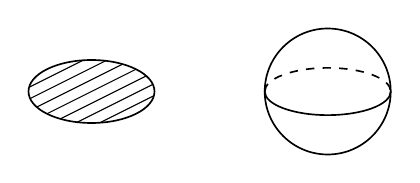
\begin{tikzpicture}[line width=.6]
    \draw (0,0) ellipse (.8 and .4);
    \begin{scope}
        \clip (0,0) ellipse (.8 and .4);
        \draw[thin] (1.7,.4) -- (.1,-.4)
                    (1.4,.4) -- (-.2,-.4)
                    (1.1,.4) -- (-.5,-.4)
                    (.8,.4) -- (-.8,-.4)
                    (.5,.4) -- (-1.1,-.4)
                    (.2,.4) -- (-1.4,-.4)
                    (-.1,.4) -- (-1.7,-.4);
    \end{scope}
    \draw (3,0) circle (.8);
    \draw[dashed] (2.2,0) arc (180:0:.8 and .3);
    \draw (2.2,0) arc (180:360:.8 and .3);
\end{tikzpicture} \]

This theorem is often proved as a consequence of
the uniformisation theorem of Riemann surfaces,
using the fact that every Riemannian $2$-manifold can be given isothermal coordinates
so that it becomes a Riemann surface.
Here we give it a new and direct proof.

\begin{proof}
By (\ref{cor:handle-decomp}) the manifold is diffeomorphic to a good $2$-handlebody $N$.
By (\ref{prop:0-handle}) we may assume it is a good weak handlebody with only one $0$-handle.
Consider the handle chain complex with $\Z_2$ coefficients
\[ \cdots\to0\to C_2(N;\Z_2)\xrightarrow{\partial_2}C_1(N;\Z_2)\xrightarrow{\partial_1}\Z_2. \]
Since $H_0(N;\Z_2)\simeq\Z_2$, we have $\partial_1=0$.
Since $N$ is simply connected, $H_1(N;\Z_2)=0$. Thus $\partial_2$ is surjective.
Note that the belt of a $1$-handle is $S^0$, i.e.\ two points.
Since $\partial_2$ is surjective,
these two points must intersect with either (a) two different $2$-handles,
or (b) only one $2$-handle in one point.
Thus we have a graph $G$,
with vertices corresponding to the $2$-handles,
and edges corresponding to $1$-handles in case (a).
For each $1$-handle in case (b), we add an ``external edge'' that connects one vertex with ``infinity''.
This can be interpreted as an infinite sequence of vertices and edges,
so that $G$ is rigorously a graph.
This graph is locally finite, and does not have \term{loops}
(i.e.\ edges whose endpoints are the same vertex).

We take a maximal tree in each connected component of $G$,
and then apply (\ref{thm-cancel-weak}) in the form of (\ref{thm:cancel-infinite}).
The effect is that these trees are collapsed.
By the same reason as above, the collapsed graph will not have loops.
Thus the resulting graph will have no edges.
This means that the resulting weak handlebody has no $1$-handles.
Therefore, if it has a $2$-handle, then it is the sphere;
if not, then it is the open disk.
\end{proof}

\begin{corollary}
    $\R^2$ has a unique smooth structure. \qed
\end{corollary}

This method generalises to prove the following.

\begin{theorem}\label{thm:2-mfd-noncompact}
Every connected non-compact $2$-manifold is diffeomorphic to a weak $(2,1)$-handlebody.
\end{theorem}

\begin{proof}
Similarly, the manifold is diffeomorphic to a good weak $2$-handlebody $N$
with only one $0$-handle.
We construct something like a graph, denoted $G$, in the same way,
except that edges ($1$-handles) need not have vertices ($2$-handles) as their endpoints.
We ignore those edges with no endpoints for a while,
and collapse maximal trees of connected components of the remaining part of $G$.
The resulting thing should be a collection of vertices,
each possibly with some loops attached to it,
and some isolated edges.

We need to show that there are actually no vertices.
Suppose the contrary. Then at some stage,
a first $2$-handle will be attached to a (non-weak)
$(2,1)$-handlebody with only one $0$-handle.
Since every edge is a loop, it follows that whenever the image of the attaching map
passes through a $1$-handle, it passes through both sides of it.
By an elementary argument in combinatorics, if it passes through a $1$-handle,
then it will pass through the whole boundary.
This means that there will be no boundary after this attaching,
and thus $N$ must be compact, a contradiction.
\end{proof}

Together with the following well-known result,
the preceding theorem will give a classification for
all boundaryless $2$-manifolds with finite topology.

The following well-known result will also be proved in our handle-theoretic way.

\begin{theorem}[Classification of closed surfaces]
Every connected closed $2$-manifold is diffeomorphic to one of the following.
\begin{enum}
\item The orientable surface $\Sigma_g:=$ connected sum of $g$ tori,
where $g=0,1,\dotsc$ \emph{(where $\Sigma_0:=S^2$)}, with Euler characteristic $\chi(\Sigma_g)=2-2g$.
\item The non-orientable surface $\Pi_k:=$ connected sum of $k$ projective planes,
where $k=1,2,\dotsc$, with Euler characteristic $\chi(\Pi_k)=2-k$.
\end{enum}
\end{theorem}

\begin{proof}
Let $N$ be a good handle decomposition.
By (\ref{prop:0-handle}), we assume that $N$ has only one $0$-handle.
Taking the dual handlebody, we may assume $N$ has only one $2$-handle.
Let $k$ denote the number of $1$-handles, and we prove by induction on $k$
that the diffeomorphism type is decided by orientability and $k$.

If $k=0$, then $N\simeq S^2$. If $k=1$, an easy argument yields $N\simeq\R P^2$.
Next we suppose $k\geq2$.
If we remove the $2$-handle, we get a $(2,1)$-handlebody with boundary $S^1$.
If we remove one more $1$-handle, one of the following happens.

(i) The boundary is two circles, and the surface is orientable.
Thus the original surface is recovered by attaching a cylinder $S^1\times I$ along these circles,
and the orientability of the original surface decides how (regarding orientation) to attach this cylinder.
If we instead attach two $2$-handles along these circles,
then the Euler characteristic will increase by $2$.
By the inductive hypothesis, the resulting surface $S$ is decided by $k$.
By (\ref{prop:move-disk}) and (\ref{cor:isotopy-ext}),
if we take two disjoint disks on $S$ and remove their interiors,
then the resulting surface $S'$ is unique up to a diffeomorphism.
Thus our original surface is decided by $k$.

(ii) The boundary is two circles, and the surface is non-orientable.
This case is the same as (i) except that by (\ref{prop:move-disk}),
the two ways (regarding orientation) of attaching a cylinder result in the same surface.

(iii) The boundary is one circle.
In this case the original surface must be non-orientable,
and will be recovered by attaching a M\"obius band along the circle.
If we instead attach a $2$-handle along the circle,
then the Euler characteristic increases by $1$.
By a same argument as in (i),
it remains to show that the connected sum $\Sigma_g\mathbin\#\Pi_1$
is diffeomorphic to $\Pi_{2g}\mathbin\#\Pi_1\simeq\Pi_{2g+1}$.
This follows from the observation that $\Pi_3\simeq\Sigma_1\mathbin\#\Pi_1$.
\end{proof}

Now we may apply our results to non-compact manifolds.
We say a manifold has \term{finite topology},
if its (say $\R$-coefficient) homology groups are finite dimensional.

\begin{theorem}[Classification of $2$-manifolds]
Every connected boundaryless $2$-manifold with finite topology
is diffeomorphic to either one of the closed surfaces $\Sigma_g$ and $\Pi_k$,
or one of them with a finite number of points removed.
\end{theorem}

\begin{proof}
The compact case follows from the preceding theorem.
For the non-compact case, by (\ref{thm:2-mfd-noncompact}),
the manifold must be a weak $(2,1)$-handlebody with one $0$-handle.
By the finiteness assumption, it must have finitely many $1$-handles.
Thus it is the interior of a finite $(2,1)$-handlebody,
whose boundary is a compact $1$-manifold, i.e.\ a finite number of circles.
After attaching $2$-handles along these circles,
it would become a closed surface, whence the result follows.
\end{proof}

The remaining case to a complete classification of $2$-manifolds
is that of weak $(2,1)$-handlebodies
with one $0$-handle and infinitely many $1$-handles.
However, classifying them is very difficult,
and even the open subsets of $\R^2$ can not easily be classified.
On the other hand, we can obtain partial results.
For example, using the results in this paper, one can show that
after multiplying by $\R$,
all the orientable ones will become diffeomorphic $3$-dimensional manifolds.


\section*{Acknowledgements}

This paper is a revision of my midterm project
for the course \emph{Algebraic Topology}
taught by professor Si Li in the spring of 2018.
I would like to thank professor Yi Jiang and professor Si Li 
for their help and suggestions.

\printbibliography

\end{document}

